\documentclass[iicol, sn-basic, Numbered]{sn-jnl} % can use "referee" option for double line spacing, "lineno" for line numbers
% template from https://www.springernature.com/gp/authors/campaigns/latex-author-support

\usepackage[ruled,linesnumbered,vlined]{algorithm2e} % pseudo-code
\usepackage{amsmath} % mathematical symbols; used by us and required by SN template class (else "Undefined control sequence. \begin{document}")
\usepackage{amssymb} % mathematical symbols
\usepackage{amsthm} % theorems, definitions etc.
\usepackage{booktabs} % nicely formatted tables (with top, mid, and bottom rule)
\usepackage{graphicx} % plots
\usepackage{manyfoot} % required by SN template class (else "Undefined control sequence. \begin{document}")
\usepackage{multirow} % cells spanning multiple rows in tables
\usepackage{subcaption} % figures with multiple sub-figures and sub-captions
\usepackage{xcolor} % required by SN template class (else "Undefined control sequence. \begin{document}")
%\usepackage{hyperref} % links and URLs; loaded by SN template class

\theoremstyle{plain}
\newtheorem{proposition}{Proposition}
\theoremstyle{definition}
\newtheorem{definition}{Definition}
\newtheorem{example}{Example}

\begin{document}

\title{Alternative Feature Selection with User Control} % use an optional parameter to set short title

\author*[1]{\fnm{Jakob} \sur{Bach}}\email{jakob.bach@kit.edu}
\author[1]{\fnm{Klemens} \sur{B\"ohm}}\email{klemens.boehm@kit.edu}

\affil*[1]{\orgdiv{Department of Informatics}, \orgname{Karlsruhe Institute of Technology (KIT)}, \orgaddress{\street{Am Fasanengarten 5}, \city{Karlsruhe}, \postcode{76131}, \state{Baden-W\"urttemberg}, \country{Germany}}}

\abstract{
	Feature selection is popular for obtaining small, interpretable, yet highly accurate prediction models.
	Conventional feature-selection methods typically yield one feature set only, which does not suffice in certain scenarios.
	For example, users might be interested in finding alternative feature sets with similar prediction quality, offering different explanations of the data.
	In this article, we introduce alternative feature selection and formalize it as an optimization problem.
	In particular, we define alternatives via constraints and enable users to control the number and dissimilarity of alternatives.
	Next, we analyze the complexity of this optimization problem and show $\mathcal{NP}$-hardness.
	Further, we discuss how to integrate conventional feature-selection methods as objectives.
	Finally, we evaluate alternative feature selection in comprehensive experiments with 30 datasets representing binary-classification problems.
	We observe that alternative feature sets may indeed have high prediction quality, and we analyze factors influencing this outcome.
}

\keywords{feature selection, alternatives, constraints, mixed-integer programming, explainability, interpretability, XAI}

\maketitle

\section{Introduction}
\label{sec:afs:introduction}

\paragraph{Motivation}

Feature-selection methods are ubiquitous for a variety of reasons.
By reducing the dimensionality of datasets, they lower the computational cost and the memory requirements of prediction models.
Prediction models also tend to generalize better without irrelevant and spurious predictors.
While some model types can implicitly select relevant features, others cannot.
In addition, simpler prediction models improve interpretability~\cite{li2017feature}.

Most conventional feature-selection methods return one feature set only~\cite{borboudakis2021extending}.
These methods optimize a criterion of feature-set quality, e.g., prediction performance.
However, besides the optimal feature set, there might be other, differently composed feature sets with similar quality.
Such alternative feature sets are interesting for users, e.g., to obtain several diverse explanations.
Alternative explanations can provide additional insights into predictions, enable users to develop and test different hypotheses, appeal to different kinds of users, and foster trust in the predictions~\cite{kim2021multi, wang2019designing}.

For example, in a dataset describing physical experiments, feature selection may help to discover relationships between physical quantities.
In particular, highly predictive feature sets indicate which input quantities are strongly related to the output quantity.
Domain experts may use these feature sets to formulate hypotheses on physical laws.
However, if multiple alternative sets of similar quality exist, further analyses and experiments may be necessary to reveal the true underlying physical mechanism.
Only knowing one predictive feature set and using it as the only explanation is misleading in such a situation.

\paragraph{Problem statement}

This article\footnote{
	This article is a polished and shortened version of a preprint available on \emph{arXiv}~\cite{bach2023finding}.
	Experimental results are the same.
}
addresses the problem of alternative feature selection, which we informally define as follows:
Find multiple, sufficiently different feature sets that optimize feature-set quality.
We provide formal definitions in Section~\ref{sec:afs:approach:constraints}.
This problem entails an interesting trade-off:
Depending on how different the alternatives should be, one may have to compromise on quality.
In particular, a stronger dissimilarity requirement may require selecting more low-quality features in the alternatives.
Users should be able to control the dissimilarity and hence this trade-off.

\paragraph{Related work}

In the field of feature selection, only a few methods yield multiple, diverse feature sets~\cite{borboudakis2021extending}.
In particular, there are techniques for ensemble feature selection~\cite{saeys2008robust, seijo2017ensemble} and statistically equivalent feature subsets~\cite{lagani2017feature}. 
These approaches do not guarantee the diversity of the feature sets, nor do they let users control diversity.
Obtaining multiple, diverse solutions also is an objective in other fields, e.g., for clustering~\cite{bailey2014alternative, hu2018subspace, mueller2009relevant}, subgroup discovery~\cite{leeuwen2012diverse}, subspace search~\cite{trittenbach2019dimension}, and explainable AI~\cite{artelt2022even, kim2016examples, russell2019efficient}.
These approaches are not directly applicable or easily adaptable to feature selection, and most of them provide limited or no user control over alternatives, as we will elaborate in Section~\ref{sec:afs:related-work}.

\paragraph{Contributions}

Our contribution is fourfold.

(1) We formalize alternative feature selection as an optimization problem.
In particular, we define alternatives via constraints on feature sets.
This approach is orthogonal to the feature-selection method itself. 
As a wide variety of such methods exists~\cite{chandrashekar2014survey, li2017feature}, users can choose a method according to their needs/preferences. 
This approach also allows integrating other constraints on feature sets, e.g., to capture domain knowledge \cite{bach2022empirical, groves2015toward}.
Finally, this approach gives users control over the search for alternatives with two parameters, i.e., the number of alternatives and a dissimilarity threshold. 

(2) We analyze the computational complexity of this problem.
We show $\mathcal{NP}$-hardness, for a simple notion of feature-set quality already. 
On the other hand, the runtime is polynomial if the sizes of the feature sets and the number of alternatives are fixed.

(3) We study how to solve this optimization problem. 
Specifically, we describe how to integrate conventional feature-selection methods into the objective function.
The resulting optimization problems are either white-box, which one can tackle with an integer-programming optimizer, or black-box, for which we propose a constraint-aware heuristic search procedure.

(4) We evaluate alternative feature selection with comprehensive experiments.
We use 30 datasets representing binary-classification problems from the Penn Machine Learning Benchmarks (PMLB)~\cite{olson2017pmlb, romano2021pmlb} and five feature-selection methods. 
We focus on the feature-set quality of alternatives relative to the user parameters.
We publish all our code\footnote{\url{https://github.com/Jakob-Bach/Alternative-Feature-Selection}} and experimental data\footnote{\url{https://doi.org/10.35097/1975}} online.

\paragraph{Experimental results}

We observe that several factors influence the quality of alternatives, namely the dataset, the feature-selection method, the notion of feature-set quality, and user parameters controlling the search for alternatives.
We have come up with several observations and recommendations, such as:
(a) Quality-wise, the prediction performance of feature sets may not correlate with the quality assigned by feature-selection methods.
In particular, seemingly bad alternatives regarding the latter might still be good regarding the former.
(b) As feature-set quality tends to decrease with an increasing number of alternatives and with an increasing dissimilarity threshold, these parameters let users indeed control the trade-off between the diversity of feature sets and their quality.
If the parameter values are too strict, no valid alternatives might even exist.
(c) Computationally, a sequential search for alternatives has turned out to be significantly faster than searching for multiple alternatives simultaneously while yielding a similar quality.

\paragraph{Outline}

Section~\ref{sec:afs:fundamentals} introduces notation and fundamentals.
Section~\ref{sec:afs:approach} describes and analyzes alternative feature selection.
Section~\ref{sec:afs:experimental-design} outlines our experimental design. 
Section~\ref{sec:afs:evaluation} presents the experimental results.
Section~\ref{sec:afs:related-work} reviews related work.
Section~\ref{sec:afs:conclusion} concludes.
Appendix~\ref{sec:afs:appendix} contains technical details and some of the proofs.

\section{Fundamentals}
\label{sec:afs:fundamentals}

In this section, we introduce basic notation (Section~\ref{sec:afs:fundamentals:notation}) and review different methods to measure the quality of feature sets (Section~\ref{sec:afs:fundamentals:quality}).

\subsection{Notation}
\label{sec:afs:fundamentals:notation}

$X \in \mathbb{R}^{m \times n}$ is a dataset represented as a matrix.
Each row is a data object, and each column is a feature.
$\tilde{F} = \{f_1, \dots, f_n\}$ is the set of feature names.
We assume that categorical features have been encoded numerically, e.g., via one-hot encoding.
$X_{\cdot{}j} \in \mathbb{R}^m$ denotes the vector representation of the $j$-th feature.
$y \in Y^m$ represents the prediction target with domain $Y$, e.g., $Y=\{0,1\}$ for binary classification or $Y=\mathbb{R}$ for regression.
Feature selection makes a binary decision $s_j \in \{0,1\}$ for each feature, i.e., either selects it or not.
The vector $s \in \{0,1\}^n$ combines all these selection decisions and yields the selected feature set $F_s = \{f_j \mid s_j=1\} \subseteq \tilde{F}$.
To simplify notation, we drop the subscript~$s$ in definitions where we do not explicitly refer to the value of~$s$ but only the set~$F$.
The function $Q(s,X,y)$ denotes the feature-set quality, which, without loss of generality, should be maximized.

\subsection{Measuring Feature (Set) Quality}
\label{sec:afs:fundamentals:quality}

There are different ways to evaluate feature-set quality $Q(s,X,y)$.
We only give a short overview here; see~\cite{chandrashekar2014survey, li2017feature, njoku2023wrapper} for comprehensive studies and surveys of feature selection.
Also, note that we assume a supervised feature-selection scenario, i.e., feature-set quality depending on a prediction target~$y$.
In principle, our definitions of alternatives also apply to an unsupervised scenario.
Since the prediction target only appears in the function~$Q(s,X,y)$, one could replace~$Q(s,X,y)$ with $Q(s,X)$, i.e., an unsupervised notion of quality.

A conventional categorization of feature-selection methods distinguishes between filter, wrapper, and embedded methods~\cite{guyon2003introduction}.
\emph{Filter methods} evaluate feature-set quality without prediction models.
Univariate filters assess each feature independently, e.g., using the correlation of the feature with the prediction target.
Multivariate filters, like CFS~\cite{hall1999correlation, hall2000correlation}, FCBF~\cite{yu2003feature}, and mRMR~\cite{peng2005feature}, assess feature sets as a whole, also considering interactions like redundancies between features.
\emph{Wrapper methods}~\cite{kohavi1997wrappers} search over feature sets with a black-box optimization strategy, e.g., genetic algorithms, and assess feature-set quality with prediction models trained on candidate feature sets.
\emph{Embedded methods} train prediction models with built-in feature selection, e.g., decision trees~\cite{breiman1984classification} or random forests~\cite{breiman2001random}.
Thus, the criterion for feature-set quality is model-specific.

Besides conventional feature selection, \emph{post-hoc feature importance methods} play a major role in the field of machine-learning interpretability~\cite{carvalho2019machine, molnar2020interpretable}.
These methods assess feature importance after training a prediction model and can be instance-specific, like LIME~\cite{ribeiro2016should} or SHAP~\cite{lundberg2017unified}, or describe the entire dataset, like permutation importance~\cite{breiman2001random} or SAGE~\cite{covert2020understanding}.

\section{Alternative Feature Selection}
\label{sec:afs:approach}

In this section, we introduce and analyze alternative feature selection.
First, we define the overall structure of the optimization problem, i.e., objective and constraints (Section~\ref{sec:afs:approach:problem}).
Second, we formalize the notion of alternatives via constraints (Section~\ref{sec:afs:approach:constraints}).
Third, we discuss different objective functions corresponding to different feature-set quality measures from Section~\ref{sec:afs:fundamentals:quality}.
In particular, we describe how to solve the resulting optimization problem (Section~\ref{sec:afs:approach:objectives}).
Fourth, we analyze the computational complexity of the optimization problem (Section~\ref{sec:afs:approach:complexity}).

\subsection{Optimization Problem}
\label{sec:afs:approach:problem}

Alternative feature selection has two goals.
First, the quality of alternatives should be high.
Second, alternative feature sets should differ from each other, i.e., contain different features.
There are different ways to combine two goals in an optimization problem:
First, one can consider both goals as objectives in a multi-objective problem.
Second, one can treat one goal as the objective and enforce the other with constraints.
Third, one can define constraints for both goals, searching for feasible solutions instead of optimizing. 
We stick to the second formulation and maximize feature-set quality subject to feature sets being alternative.
This formulation allows us to keep the original objective function of feature selection.
Thus, users do not need to specify a threshold on feature-set quality but control how alternative the feature sets must be instead.
We obtain the following optimization problem (Equation~\ref{eq:afs:afs-general}) to find a single alternative feature set~$F_s$:
%
\begin{equation}
	\begin{aligned}
		\max_s &\quad Q(s,X,y) \\
		\text{subject to:} &\quad F_s~\text{being alternative}
	\end{aligned}
	\label{eq:afs:afs-general}
\end{equation}
%
In the following, we discuss different objective functions $Q(s,X,y)$ and suitable constraints for \emph{being alternative}.
Additionally, many feature-selection methods limit the feature-set size $|F_s|$ to a user-defined value~$k \in \mathbb{N}$, which adds further, simple constraints.

\subsection{Constraints -- Defining Alternatives}
\label{sec:afs:approach:constraints}

We now formalize alternative feature sets via constraints, considering single (Section~\ref{sec:afs:approach:constraints:single}) and multiple alternatives (Section~\ref{sec:afs:approach:constraints:multiple}).
All our definitions are independent of the feature-selection method.

\subsubsection{Single Alternative}
\label{sec:afs:approach:constraints:single}

We consider a feature set an alternative to another set if it differs sufficiently.
We express this notion with a set-dissimilarity measure~\cite{choi2010survey, egghe2009new}.
These measures typically quantify how strongly two sets $F'$, $F''$ overlap and relate this to their sizes.
For instance, a well-known set-dissimilarity measure is the Jaccard distance, which is defined as follows (Equation~\ref{eq:afs:jaccard}) for the feature sets $F'$ and $F''$:
%
\begin{equation}
	\begin{aligned}
		d_{\text{Jacc}}(F',F'') & = 1 - \frac{|F' \cap F''|}{|F' \cup F''|} \\
		& = 1 - \frac{|F' \cap F''|}{|F'| + |F''| - |F' \cap F''|}
	\end{aligned}
	\label{eq:afs:jaccard}
\end{equation}
%
In this article, we use a dissimilarity measure based on the Dice coefficient, as defined by Equation~\ref{eq:afs:dice}:
%
\begin{equation}
	d_{\text{Dice}}(F',F'') = 1 - \frac{2 \cdot |F' \cap F''|}{|F'| + |F''|}
	\label{eq:afs:dice}
\end{equation}
%
Other measures are also possible.
Our definitions of alternatives only assume non-negativity, i.e., $d(F',F'') \geq 0$, and symmetry, i.e., $d(F',F'')=d(F'',F')$.
We define single alternatives as follows:
%
\begin{definition}[Single alternative]
	Given a symmetric, non-negative set-dissimilarity measure~$d(\cdot)$ and a dissimilarity threshold~$\tau \in \mathbb{R}_{\geq 0}$, a feature set $F'$ is an alternative to a feature set~$F''$ (and vice versa) if $d(F',F'') \geq \tau$.
	\label{def:afs:single-alternative}
\end{definition}
%
The threshold~$\tau$ controls how dissimilar alternative feature sets should be.
The larger~$\tau$, the more feature-set quality may drop.
However, depending on the dataset, the same value of~$\tau$ may have a stronger or weaker effect on feature-set quality.
For example, certain datasets may encompass numerous features with similar levels of utility, thereby allowing for numerous alternatives of comparable quality. 
In contrast, predictions on other datasets may hinge on a few key features.
Further, only users can decide which drop in feature-set quality is acceptable as a trade-off for obtaining alternatives.
Thus, we leave $\tau$ as a user parameter.
For normalized dissimilarity measures as in Equations~\ref{eq:afs:jaccard} and~\ref{eq:afs:dice}, the interpretation of $\tau$ is user-friendly:
Setting $\tau=0$ allows identical alternatives, while $\tau=1$ forbids any overlap.
Users can also experiment with various values, such as performing a binary search across the range of~$\tau$.

When implementing Definition~\ref{def:afs:single-alternative}, the following proposition gives way to using a broad range of solvers to tackle the related optimization problem:
%
\begin{proposition}[Linearity of constraints]
	Using the Dice dissimilarity (Equation~\ref{eq:afs:dice}), one can express alternative feature sets (Definition~\ref{def:afs:single-alternative}) with 0-1 integer linear constraints.
	\label{prop:afs:linear-constraints}
\end{proposition}
%
\begin{proof}
We re-arrange terms in the Dice dissimilarity (Equation~\ref{eq:afs:dice}) to get rid of the quotient of feature-set sizes, obtaining Equation~\ref{eq:afs:dice-rearranged}:
%
\begin{equation}
	\begin{aligned}
		& & d_{\text{Dice}}(F',F'') & \geq \tau \\
		& \Leftrightarrow & |F' \cap F''| & \leq \frac{1 - \tau}{2} \cdot (|F'| + |F''|)
	\end{aligned}
	\label{eq:afs:dice-rearranged}
\end{equation}
%
Next, we express set sizes in terms of the feature-selection vector $s$, obtaining Equation~\ref{eq:afs:feature-set-size}:
%
\begin{equation}
	\begin{aligned}
		|F_s| & = \sum_{j=1}^n s_j \\
		|F_{s'} \cap F_{s''}| & = \sum_{j=1}^n s'_j \cdot s''_j
	\end{aligned}
	\label{eq:afs:feature-set-size}
\end{equation}
%
Finally, we replace each product $s'_j \cdot s''_j$ with an auxiliary variable~$t_j$, bound by additional constraints, to linearize it~\cite{mosek2022modeling}, obtaining Equation~\ref{eq:afs:product-linear}:
%
\begin{equation}
	\begin{aligned}
		t_j & \leq s'_j \\
		t_j & \leq s''_j \\
		1 + t_j & \geq s'_j + s''_j \\
		t_j & \in \{0,1\}
	\end{aligned}
	\label{eq:afs:product-linear}
\end{equation}
%
Only sums of variables and products with constants remain, so the constraints are linear.
Further, if one feature set is known, i.e., either $s'$ or $s''$ is fixed to particular values, Equation~\ref{eq:afs:feature-set-size} already is linear without Equation~\ref{eq:afs:product-linear}.
\end{proof}
%
As an alternative formulation, one could also encode the 0-1 integer linear constraints into propositional logic (\textsc{SAT})~\cite{ulrich2022selecting}.

If the set sizes $|F'|$ and $|F''|$ are constant, e.g., user-defined, Equation~\ref{eq:afs:dice-rearranged} implies that the threshold~$\tau$ exhibits a linear relationship with the maximum number of overlapping features~$|F' \cap F''|$.
This correspondence simplifies the interpretation of~$\tau$ and encourages us to utilize the Dice dissimilarity in the subsequent steps.
On the contrary, the Jaccard distance exhibits a non-linear relationship between $\tau$ and the overlap size.
This insight arises from rearranging Equation~\ref{eq:afs:jaccard} in conjunction with Definition~\ref{def:afs:single-alternative}, obtaining Equation~\ref{eq:afs:jaccard-rearranged}:
%
\begin{equation}
	\begin{aligned}
		d_{\text{Jacc}}(F',F'') & = 1 - \frac{|F' \cap F''|}{|F'| + |F''| - |F' \cap F''|} \geq \tau \\
		& \Leftrightarrow |F' \cap F''| \leq \frac{1 - \tau}{2 - \tau} \cdot (|F'| + |F''|)
	\end{aligned}
	\label{eq:afs:jaccard-rearranged}
\end{equation}
%
Further, if $|F'| = |F''|$, Equation~\ref{eq:afs:dice-rearranged} implies that parameter~$\tau$ represents the share of features in one set that must not be a member of the other one, and vice versa, as expressed by Equation~\ref{eq:afs:dice-rearranged-equal-size}:
%
\begin{equation}
	\begin{aligned}
		& & d_{\text{Dice}}(F',F'') & \geq \tau \\
		& \Leftrightarrow & |F' \cap F''| & \leq (1 - \tau) \cdot |F'| \\
		& & & = (1 - \tau) \cdot |F''|
	\end{aligned}
	\label{eq:afs:dice-rearranged-equal-size}
\end{equation}
%
This correspondence further eases interpretability.
In particular, if users are uncertain how to choose $\tau$, and if $|F'|$ is reasonably small, users can try out all values of $\tau \in \{i / |F'|\}$ with $i \in \{1, \dots, |F'|\}$.
These $|F'|$~unique values of $\tau$ suffice to produce all possible distinct solutions that one could obtain with an arbitrary $\tau \in (0,1]$.

\subsubsection{Multiple Alternatives}
\label{sec:afs:approach:constraints:multiple}

One can search for multiple alternatives either sequentially or simultaneously.
The number of alternatives~$a \in \mathbb{N}_0$ is a parameter for the users.
The overall number of feature sets is~$a+1$ since we deem one feature set the `original' one.
Table~\ref{tab:afs:seq-sim-comparison} compares the sizes of the optimization problems for these two search methods.

\begin{table*}[t]
	\centering
	\renewcommand*{\arraystretch}{1.3} % spacing between lines in table (increase due to use of \frac in rows)
	\begin{tabular}{lccc}
		\toprule
		& \multicolumn{2}{c}{Sequential search} & \multirow{2}{*}{Simultaneous search} \\
		\cmidrule(r){2-3}
		& Alternative $i$ & Summed & \\
		\midrule
		Decision variables~$s$ & $n$ & $ (a+1) \cdot n$ & $(a+1) \cdot n$ \\
		Linearization variables~$t$ & $0$ & $0$ & $\frac{a \cdot (a+1) \cdot n}{2}$ \\
		Alternative constraints & $i$ & $\frac{a \cdot (a+1)}{2}$ & $\frac{a \cdot (a+1)}{2}$ \\
		Linearization constraints & $0$ & $0$ & $\frac{3 \cdot a \cdot (a+1) \cdot n}{2}$ \\
		\bottomrule
	\end{tabular}
	\caption{Size of the optimization problem by search method, for $a$~alternatives ($a + 1$~feature sets overall) and $n$ features.}
	\label{tab:afs:seq-sim-comparison}
\end{table*}

\paragraph{Sequential alternatives}

With sequential search, users obtain alternatives iteratively, with one alternative per iteration.
Thus, users can monitor the quality of alternatives and end the search after each iteration.
This option frees users from setting the parameter~$a$ a priori.
Each feature set has to be an alternative to all previously found ones, which are contained within the set~$\mathbb{F}$:
%
\begin{definition}[Sequential alternative]
	A feature set~$F''$ is an alternative to a set of feature sets~$\mathbb{F}$ (and vice versa) if $F''$ is a single alternative (Definition~\ref{def:afs:single-alternative}) to each $F' \in \mathbb{F}$.
	\label{def:afs:sequential-alternative}
\end{definition}
%
Adapting Equation~\ref{eq:afs:afs-general} to Definition~\ref{def:afs:sequential-alternative}, we obtain the following optimization problem (Equation~\ref{eq:afs:afs-sequential}) for each iteration of the search:
%
\begin{equation}
	\begin{aligned}
		\max_s &\quad Q(s,X,y) \\
		\text{subject to:} &\quad \forall F' \in \mathbb{F}:~d(F_s,F') \geq \tau
	\end{aligned}
	\label{eq:afs:afs-sequential}
\end{equation}
%
The objective function remains the same as for a single alternative, i.e., optimizes only one feature set~$F_s$ per iteration.
In particular, with $\mathbb{F} = \emptyset$ in the first iteration, we optimize for the `original' feature set, which is the same as in conventional feature selection without constraints for alternatives.
Thus, the number of variables in each optimization is independent of the number of alternatives~$a$, and no linearization variables (Equation~\ref{eq:afs:product-linear}) are required.
Each alternative only adds one new constraint to the problem.
Thus, we expect the runtime of sequential search to scale well with the number of alternatives.
Additional runtime improvements can be achieved if the optimizer retains a state between iterations and can warm-start.

\paragraph{Simultaneous alternatives}

Through simultaneous search, users can acquire multiple alternatives simultaneously, whose number~$a$ must be set beforehand.
Once more, we employ pairwise dissimilarity constraints for these alternatives:
%
\begin{definition}[Simultaneous alternatives]
	A set of feature sets~$\mathbb{F}$ contains simultaneous alternatives if each feature set~$F' \in \mathbb{F}$ is a single alternative (Definition~\ref{def:afs:single-alternative}) to each other set~$F'' \in \mathbb{F}$, $F' \neq F''$.
	\label{def:afs:simultaneous-alternative}
\end{definition}
%
Adapting Equation~\ref{eq:afs:afs-general} to Definition~\ref{def:afs:simultaneous-alternative}, we obtain the following optimization problem (Equation~\ref{eq:afs:afs-simultaneous}):
%
\begin{equation}
	\begin{aligned}
		\max_{s^{(0)}, \dots, s^{(a)}} &\quad \operatorname*{agg}_{i \in \{0, \dots, a\}} Q(s^{(i)},X,y) \\
		\text{subject to:} &\quad \forall i_1, i_2 \in \{0, \dots, a\},~i_1 \neq i_2: \\
		& \quad\quad d(F_{s^{(i_1)}},F_{s^{(i_2)}}) \geq \tau
	\end{aligned}
	\label{eq:afs:afs-simultaneous}
\end{equation}
%
In contrast to the sequential case (Equation~\ref{eq:afs:afs-sequential}), the problem requires a modified objective function and $a+1$ instead of one decision vector~$s$.
The operator~$\text{agg}(\cdot)$ defines how to aggregate the qualities of the feature sets.
In our experiments, we consider the sum as well as the minimum to instantiate~$\text{agg}(\cdot)$, which we refer to as \emph{sum-aggregation} and \emph{min-aggregation}.
The latter explicitly fosters balanced feature-set qualities.
Appendix~\ref{sec:afs:appendix:simultaneous-objective-aggregation} discusses these two aggregation operators and additional ideas for balancing qualities in detail.

In terms of runtime, we anticipate simultaneous search to scale worse with the number of alternatives~$a$ than sequential search. 
This is because simultaneous search addresses a single large optimization problem, as opposed to several smaller ones. 
The number of decision variables grows linearly with~$a$, while the number of constraints increases quadratically.
Further, auxiliary variables are necessary to obtain linear constraints (Equation~\ref{eq:afs:product-linear}).

Quality-wise, simultaneous search may benefit from optimizing once rather than greedily.
Furthermore, the quality may be distributed more evenly across the alternatives compared to sequential search.
However, a drawback is that there are no intermediate steps where users can interrupt the search after assessing the current feature-set quality.

\subsection{Objective Functions -- Finding Alternatives}
\label{sec:afs:approach:objectives}

In this section, we delve into the process of identifying alternative feature sets.
Specifically, we describe how to solve the optimization problem introduced in Section~\ref{sec:afs:approach:problem} for the different categories of feature-set quality measures featured in Section~\ref{sec:afs:fundamentals:quality}.
We distinguish between white-box (Section~\ref{sec:afs:approach:objectives:white-box}), black-box (Section~\ref{sec:afs:approach:objectives:black-box}), and embedding (Section~\ref{sec:afs:approach:objectives:embedding}) approaches.

\subsubsection{White-Box Optimization}
\label{sec:afs:approach:objectives:white-box}

If the feature-set quality function $Q(s,X,y)$ is sufficiently simple, one can find alternatives with a solver for white-box optimization problems.
We already showed that our notion of alternative feature sets can be expressed as 0-1 integer linear constraints (Proposition~\ref{prop:afs:linear-constraints}).
We now discuss four popular feature-selection methods with objectives that admit formulating a 0-1 integer linear problem.
We evaluate all four methods in our experiments later.

\paragraph{Univariate filter feature selection}

For univariate filter methods, the objective function is linear by default since the quality of a feature set is the sum of the qualities of the individual features, as defined by Equation~\ref{eq:afs:univariate-filter}:
%
\begin{equation}
	Q_{\text{uni}}(s,X,y) = \sum_{j=1}^{n} q(X_{\cdot{}j},y) \cdot s_j
	\label{eq:afs:univariate-filter}
\end{equation}
%
Here, $q(\cdot)$ is a bivariate dependency measure to quantify the relationship between each feature and the prediction target, e.g., mutual information~\cite{kraskov2004estimating} or the absolute value of Pearson correlation.

For this objective, Appendix~\ref{sec:afs:appendix:univariate-complete-optimization-problem} specifies the complete optimization problem, including the constraints for alternatives we already introduced in Section~\ref{sec:afs:approach:constraints}.

\paragraph{Post-hoc feature importance}

One can also insert post-hoc feature-importance scores as univariate feature qualities~$q(X_{\cdot{}j},y)$ into Equation~\ref{eq:afs:univariate-filter}.
However, such post-hoc importance scores typically evaluate the quality of each feature in the presence of other features. 
For example, a feature may only be important in subsets where another feature is present, due to feature interaction, but unimportant otherwise, and a post-hoc importance method like SHAP~\cite{lundberg2017unified} may reflect both these aspects.
In contrast, Equation~\ref{eq:afs:univariate-filter} implicitly assumes feature independence and cannot adapt importance scores depending on whether other features are selected.
Thus, treating pre-computed post-hoc importance scores as univariate feature qualities in the optimization objective can serve as a heuristic but may not faithfully represent the actual feature qualities in a particular selected set.

\paragraph{FCBF}

The Fast Correlation-Based Filter (FCBF)~\cite{yu2003feature} is a multivariate filter method based on the notion of predominance:
The correlation of each selected feature with the prediction target must exceed a user-defined threshold and must also be higher than the correlation of each other selected feature with the given one.
While FCBF originally employs a heuristic search to identify predominant features, we propose a formulation as a constrained optimization problem (Equation~\ref{eq:afs:fcbf}) to allow a white-box optimization for alternatives:
%
\begin{equation}
	\begin{gathered}
		\max_s \quad Q_{\text{FCBF}}(s,X,y) = \sum_{j=1}^{n} q(X_{\cdot{}j},y) \cdot s_j \\
		\begin{aligned}
			\text{subject to:} &\quad \forall j_1, j_2 \in \{1, \dots, n\},~j_1 \neq j_2, \\
			& \quad q(X_{\cdot{}j_1},y) \leq q(X_{\cdot{}j_2}, X_{\cdot{}j_1}): \\
			& \quad\quad s_{j_1} + s_{j_2} \leq 1 \\
		\end{aligned}
	\end{gathered}
	\label{eq:afs:fcbf}
\end{equation}
%
We drop the original FCBF's threshold on feature-target correlation and maximize the latter instead, as in the univariate-filter case.
Further, we keep the constraints of FCBF on feature-feature correlation.
Specifically, we prohibit the concurrent selection of two features if their correlation is at least as high as the correlation of either feature with the target variable. 
Since the condition~$q(X_{\cdot{}j_1},y) \leq q(X_{\cdot{}j_2}, X_{\cdot{}j_1})$ in Equation~\ref{eq:afs:fcbf} does not depend on the decision variables~$s$, one can pre-compute whether it holds before formulating the optimization problem and add the corresponding linear constraint $s_{j_1} + s_{j_2} \leq 1$ only for feature pairs where it is needed.

\paragraph{mRMR}

The multivariate filter method Minimal Redundancy Maximum Relevance (mRMR)~\cite{peng2005feature} combines two criteria, relevance and redundancy.
Relevance is the dependency between selected features and the prediction target, as for univariate filter methods. 
Redundancy, in turn, quantifies the dependency between selected features.
Both terms are averaged over the selected features.
The objective is to maximize the difference between relevance and redundancy, as defined by Equation~\ref{eq:afs:mrmr}:
%
\begin{multline}
	\max_s \quad Q_{\text{mRMR}}(s,X,y) = \frac{\sum_{j=1}^{n} q(X_{\cdot{}j},y) \cdot s_j}{\sum_{j=1}^{n} s_j} \\
	- \frac{\sum_{j_1=1}^{n} \sum_{j_2=1}^{n} q(X_{\cdot{}j_1}, X_{\cdot{}j_2}) \cdot s_{j_1} \cdot s_{j_2}}{(\sum_{j=1}^{n} s_j)^2}
	\label{eq:afs:mrmr}
\end{multline}
%
If one knows the feature-set size $\sum_{j=1}^{n} s_j$ to be a constant~$k$, the denominators of both fractions are constant, so the objective leads to a quadratic-programming problem~\cite{nguyen2014effective, rodriguez2010quadratic}.
If one additionally replaces each product terms $s_{j_1} \cdot s_{j_2}$ according to Equation~\ref{eq:afs:product-linear}, the problem becomes linear.
However, there is a more efficient linearization~\cite{nguyen2009optimizing, nguyen2010towards}, which we use in our experiments, displayed in Equation~\ref{eq:afs:mrmr-linear}:
%
\begin{equation}
	\begin{gathered}
		\begin{aligned}
			\max_s \quad Q_{\text{mRMR}}(s,X,y) = & \frac{\sum_{j=1}^{n} q(X_{\cdot{}j},y) \cdot s_j}{k} \\
			& - \frac{\sum_{j=1}^{n} z_j}{k \cdot (k-1)} \\
		\end{aligned} \\
		\begin{aligned}
			\text{s.t.:} &\quad \forall j_1: & A_{j_1} &= \sum_{j_2 \neq j_1} q(X_{\cdot{}j_1}, X_{\cdot{}j_2}) \cdot s_{j_2} \\
			&\quad \forall j: & z_j &\geq M \cdot (s_j - 1) + A_j \\
			&\quad \forall j: & z_j &\in \mathbb{R}_{\geq 0} \\
			\text{with:} &\quad & j, j_1, j_2 &\in \{1, \dots, n\}
		\end{aligned}
	\end{gathered}
	\label{eq:afs:mrmr-linear}
\end{equation}
%
Here, $A_{j_1}$ is the sum of all redundancy terms related to the feature with index~$j_1$, i.e., the summed dependency value between this feature and all other selected features.
Thus, one can use one real-valued auxiliary variable $z_j$ for each feature instead of one new binary variable for each pair of features.
Since redundancy should be minimized, $z_j$ assumes the value of $A_j$ with equality if the feature with index~$j$ is selected~($s_j=1$) and is zero otherwise ($s_j=0$).
To this end, $M$ is a large positive value that deactivates the constraint $z_j \geq A_j$ if $s_j=0$.

Since Equation~\ref{eq:afs:mrmr-linear} assumes the feature-set size~$k \in \mathbb{N}$ to be user-defined before optimization, it requires fewer auxiliary variables and constraints than the more general formulation in~\cite{nguyen2009optimizing, nguyen2010towards}.
Additionally, in accordance with~\cite{nguyen2014effective}, we assign a value of zero to the self-redundancy terms $q(X_{\cdot{}j},X_{\cdot{}j})$, effectively excluding them from the objective function.
Thus, the redundancy term uses $k \cdot (k-1)$ instead of $k^2$ for averaging.

\subsubsection{Black-Box Optimization}
\label{sec:afs:approach:objectives:black-box}

\paragraph{Overview of approaches}

If feature-set quality does not have an expression suitable for white-box optimization, one has to treat it as a black-box function when searching for alternatives.
This situation applies to wrapper feature-selection methods, which use prediction models to assess feature-set quality.
There are several ways to consider the constraints for alternatives in such scenarios:
First, one can enumerate and evaluate all feature sets satisfying the constraints, which is inefficient.
Second, one can sample from the space of valid feature sets.
However, uniform sampling from a constrained space is a computationally hard problem, possibly harder than determining if a valid solution exists or not~\cite{ermon2012uniform}.
Third, one can formulate a multi-objective problem to avoid hard constraints on alternatives.
However, as explained in Section~\ref{sec:afs:approach:problem}, we decided to pursue a single-objective formulation with constraints.
Fourth, one can push constraints into a search heuristic; this is what we describe next.
One idea is to prevent the heuristic from producing invalid feature sets or to make this less likely, e.g., by adding a penalty to the objective function.
Another idea is to `repair' invalid feature sets in the search, e.g., by replacing them with the most similar feature sets satisfying the constraints.
Such solver-assisted approaches are popular for finding valid software configurations~\cite{guo2018preserve, henard2015combining, white2010automated}.
In our experiments, we also employ a repair-based approach, which we describe in the following.

\begin{algorithm*}[t]
	\DontPrintSemicolon
	\KwIn{Dataset $X$ with $n$ features, \newline
		Prediction target $y$, \newline
		Feature-set quality function $Q(\cdot)$, \newline
		Constraints for alternatives $Cons$, \newline
		Maximum number of iterations $max\_iters$}
	\KwOut{Set of feature-selection decision vectors $S = \{s^{(0)}, \dots, s^{(a)}\}$}
	\BlankLine
	$S \leftarrow \text{Solve}(Cons)$ \tcp*{Initial alternatives} \label{al:afs:greedy-wrapper:line:init}
	$iters \leftarrow 1$ \tcp*{Number of iterations = solver calls}
	\lIf(\tcp*[f]{No valid alternatives exist}){$S = \emptyset$}{\Return{$\emptyset$}}
	$j_1 \leftarrow 1$ \tcp*{Indices of features to be swapped}
	$j_2 \leftarrow j_1 + 1$\;
	\While{$iters < max\_iters$ \textbf{and} $j_1 < n$}{ \label{al:afs:greedy-wrapper:line:stop}
		$S' \leftarrow \text{Solve}(Cons \cup \{\neg s^{(i)}_{j_1}, \neg s^{(i)}_{j_2} \mid i \in \{0, \dots, a\}\})$ \tcp*{Try swap} \label{al:afs:greedy-wrapper:line:swap}
		$iters \leftarrow iters + 1$\;
		\If(\tcp*[f]{Swap if improved}){$S' \neq \emptyset$ \textbf{and} $Q(S',X,y) > Q(S,X,y)$}{ \label{al:afs:greedy-wrapper:line:improved-condition}
			$S \leftarrow S'$\; \label{al:afs:greedy-wrapper:line:improved-start}
			$j_1 \leftarrow 1$ \tcp*{Reset swap-feature indices}
			$j_2 \leftarrow j_1 + 1$\; \label{al:afs:greedy-wrapper:line:improved-end}
		}
		\ElseIf(\tcp*[f]{Try next swap; advance one index}){$j_2 < n$}{ \label{al:afs:greedy-wrapper:line:next-start}
			$j_2 \leftarrow j_2 + 1$\;
		}
		\Else(\tcp*[f]{Try next swap; advance both indices}){
			$j_1 \leftarrow j_1 + 1$\;
			$j_2 \leftarrow j_1 + 1$\; \label{al:afs:greedy-wrapper:line:next-end}
		}
	}
	\Return{$S$}
	\caption{\emph{Greedy Wrapper} for alternative feature selection.}
	\label{al:afs:greedy-wrapper}
\end{algorithm*}

\paragraph{Greedy Wrapper}

We propose a novel greedy hill-climbing procedure, displayed in Algorithm~\ref{al:afs:greedy-wrapper}.
Unlike standard hill climbing for feature selection~\cite{kohavi1997wrappers}, our procedure observes constraints.
First, the algorithm uses a solver to find one solution that is alternative enough, given the current constraints (Line~\ref{al:afs:greedy-wrapper:line:init}).
Thus, it has a valid starting point and can always return a solution unless there are no valid solutions at all.
Next, it tries `swapping' two features, i.e., selecting the features if they were deselected or deselecting them if they were selected (Line~\ref{al:afs:greedy-wrapper:line:swap}).
For simultaneous search, we swap the affected two features in each alternative feature set.
This swap might violate cardinality constraints as well as constraints for alternatives.
Thus, the algorithm calls the solver again to find one solution~$S'$ containing this swap and satisfying the other constraints.
If such a solution~$S'$ exists and its quality~$Q(S',X,y)$ is higher than the one of the current solution, the algorithm proceeds with the new solution, attempting again to swap the first and second features (Lines~\ref{al:afs:greedy-wrapper:line:improved-start}--\ref{al:afs:greedy-wrapper:line:improved-end}).
Otherwise, it tries to swap the next pair of features (Lines~\ref{al:afs:greedy-wrapper:line:next-start}--\ref{al:afs:greedy-wrapper:line:next-end}).
Specifically, we assess only one solution per swap before proceeding instead of exhaustively enumerating and evaluating all valid solutions involving the swap.

The algorithm terminates if no swap leads to an improvement or a fixed number of iterations~$max\_iters$ is reached (Line~\ref{al:afs:greedy-wrapper:line:stop}).
Due to its heuristic nature, the algorithm might get stuck in local optima rather than yielding the global optimum.
In particular, $max\_iters$ only is an upper bound on the iteration count since the algorithm can stop earlier.
We define the iteration count as the number of invocations of the solver, i.e., attempts to generate valid alternatives.
This number also bounds the number of prediction models trained.
However, we only train a model for valid solutions (Line~\ref{al:afs:greedy-wrapper:line:improved-condition}), and not all solver calls may yield one.

\subsubsection{Embedding Alternatives}
\label{sec:afs:approach:objectives:embedding}

If feature selection is embedded into a prediction model, there is no general approach for finding alternative feature sets.
Instead, one would need to embed the search for alternatives into model training as well.
Thus, we leave the formulation of specific approaches open for future work.
For instance, one could prevent decision trees from splitting on a feature if the resulting feature set is too similar to a given feature set.
As another example, there are various formal encodings of prediction models, e.g., as \textsc{SAT} formulas~\cite{narodytska2018learning, schidler2021sat, yu2021learning}.
In such representations, one might directly add the constraints for alternatives and employ a solver for `training'.

\subsection{Computational Complexity}
\label{sec:afs:approach:complexity}

In this section, we discuss the time complexity of alternative feature selection.
We are interested in scalability regarding the number of features~$n \in \mathbb{N}$, also taking the feature-set size~$k \in \mathbb{N}$ and the number of alternatives~$a \in \mathbb{N}_0$ into account.
Section~\ref{sec:afs:approach:complexity:exhaustive} examines exhaustive search, which works for arbitrary feature-selection methods, while Section~\ref{sec:afs:approach:complexity:uni} analyzes the optimization problem with univariate feature qualities (Equation~\ref{eq:afs:univariate-filter}).

\subsubsection{Exhaustive Search for Arbitrary Feature-Selection Methods}
\label{sec:afs:approach:complexity:exhaustive}

An exhaustive search over all possible feature sets is a simple but inefficient approach to finding alternatives. 
This procedure provides an upper bound for the time complexity of the optimization problem.

\paragraph{Sequential search}

Even without considering alternatives, the search space of feature selection grows exponentially with~$n$.
In particular, there are $2^n - 1$ non-empty feature sets of arbitrary size and $\binom{n}{k} = \frac{n!}{k! \cdot (n-k)!} \leq n^k$ sets of a fixed size~$k$.
These numbers also hold for sequential search (Equation~\ref{eq:afs:afs-sequential}), which optimizes alternatives one at a time.
For each feature set, one must evaluate the objective and check the constraints.
The cost of the former depends on the feature-selection method but should usually be polynomial in~$n$.
The latter entails a cost of~$O(a \cdot n)$ for each new alternative and~$O(a^2 \cdot n)$ for the whole sequential search with $a$~alternatives.
In particular, constraint checking involves iterating over all existing feature sets and features to compute the dissimilarity between sets (Equation~\ref{eq:afs:afs-sequential-complete}).
With $O(n^k)$ feature sets as solution candidates, we obtain the following proposition:
%
\begin{proposition}[Complexity of exhaustive sequential search]
	Exhaustive sequential search for $a \in \mathbb{N}$~alternative feature sets of size~$k$ from $n$~features has a time complexity of~$O(a^2 \cdot n^{k+1})$ without the cost of evaluating the objective function.
	\label{prop:afs:complexity-exhaustive-sequential}
\end{proposition}
%
This complexity is polynomial in~$n$ if $k$ is a small constant independent of~$n$, i.e., $k \in O(1)$, and if $a$ is at most polynomial in~$n$, i.e., $a \in O(n^c),~c \in O(1)$.
The assumption $k \in O(1)$ makes sense for feature selection, where one typically wants to obtain small feature sets from a high-dimensional dataset.
However, the exponent~$k$ might still render an exhaustive search practically infeasible.
In terms of parameterized complexity, the problem resides in class~$\mathcal{XP}$ since the complexity term has the form $O(f(k) \cdot n^{g(k)})$~\cite{downey1997parameterized} if~$a$ is constant, having the parameter~$k$ and functions $f(k) = 1$, $g(k) = k+1$.

\paragraph{Simultaneous search}

Simultaneous search enlarges the search space by optimizing $a+1$ feature sets at once (Equation~\ref{eq:afs:afs-simultaneous}), having~$O((n^k)^{a+1}) = O(n^{k \cdot (a+1)})$ solution candidates.
Thus, the following proposition holds:
%
\begin{proposition}[Complexity of exhaustive simultaneous search]
	Exhaustive simultaneous search for $a \in \mathbb{N}$~alternative feature sets of size~$k$ from $n$~features has a time complexity of~$O(a^2 \cdot n^{k \cdot (a+1) + 1})$ without the cost of evaluating the objective function.
	\label{prop:afs:complexity-exhaustive-simultaneous-np}
\end{proposition}
%
The scalability with respect to $n$ is less favorable compared to sequential search, as the number of alternatives~$a$ now appears in the exponent.
Further, Proposition~\ref{prop:afs:complexity-exhaustive-simultaneous-np} assumes that the constraints do not use linearization variables (Equations~\ref{eq:afs:product-linear} and~\ref{eq:afs:afs-simultaneous-complete}), which would enlarge the search space even further.
Finally, the complexity remains polynomial in~$n$ if $a$ and~$k$ are small and independent from~$n$, i.e., $a \cdot k \in O(1)$:
%
\begin{proposition}[Parameterized complexity of simultaneous search]
	Simultaneous search for $a \in \mathbb{N}$~alternative feature sets of size~$k$ from $n$~features resides in the parameterized complexity class $\mathcal{XP}$ for the parameter~$a \cdot k$.
	\label{prop:afs:complexity-simultaneous-xp}
\end{proposition}
%

\subsubsection{Univariate Feature Qualities}
\label{sec:afs:approach:complexity:uni}

While the assumption $a \cdot k \in O(1)$ ensures polynomial runtime regarding~$n$ for arbitrary feature-selection methods, the optimization problem can still be hard without this assumption.
In the following, we derive complexity results for \emph{univariate feature qualities} (Equation~\ref{eq:afs:univariate-filter}).
This feature-selection method arguably has the simplest objective function, where the quality of a feature set is equal to the sum of the individual qualities of its constituent features.
This simplicity eases the transformation from and to well-known $\mathcal{NP}$-hard problems.

In the following complexity analyses, we assume the feature qualities~$q(X_{\cdot{}j},y)$ are given.
In particular, one can pre-compute these qualities before searching alternatives and treat them as constants in the optimization problem.
The complexity of this computation depends on the particular feature-quality measure and the number of data objects~$m$.
However, the number of features~$n$ should only affect the complexity linearly due to the univariate setting.

We have previously observed that our optimization problem with univariate feature qualities can be formulated as an integer-linear program (Section~\ref{sec:afs:approach:objectives:white-box}).
While \textsc{Integer programming} is $\mathcal{NP}$-complete in general~\cite{garey2003computers, karp1972reducibility}, our problem is a special case of it and could therefore have lower complexity. 

\paragraph{Min-aggregation}

We start with two assumptions, both of which we will drop later:
First, we use a dissimilarity threshold of~$\tau = 1$, i.e., zero overlap of feature sets.
Second, all features must be part of one set.
We call the combination of these assumptions, which implies $n = (a+1) \cdot k$, a \emph{complete partitioning}.
This scenario differs from $a \cdot k \ll n$, which we assumed in Section~\ref{sec:afs:approach:complexity:exhaustive}, where runtime was polynomial in~$n$.

The currently assumed scenario is a variant of an existing problem known as \textsc{Multi-Way Number Partitioning}~\cite{lawrinenko2017identical} or \textsc{Multiprocessor Scheduling}~\cite{garey2003computers} in literature:
Partition a set of $n$~integers into a fixed number of subsets such that all subset sums are as equal as possible~\cite{korf2010objective}.
A typical application is assigning tasks with different lengths to a fixed number of processors, aiming to balance the load.
In our scenario, the tasks correspond to features, the task lengths to univariate feature qualities, and the processors to feature sets. 
Maximizing the minimum sum is one of several possible objectives in the literature~\cite{korf2010objective, lawrinenko2017identical}.
This objective corresponds to simultaneous search (Equation~\ref{eq:afs:afs-simultaneous}) with min-aggregation (Equation~\ref{eq:afs:afs-simultaneous-min-objective}) in our scenario.
Since \textsc{Multiprocessor Scheduling} is $\mathcal{NP}$-complete, even for just two partitions~\cite{garey2003computers}, we obtain the following result:
%
\begin{proposition}[Complexity of simultaneous search with min-aggregation, complete partitioning, and unconstrained feature-set size]
	Assuming univariate feature qualities (Equation~\ref{eq:afs:univariate-filter}), a dissimilarity threshold~$\tau = 1$, and unconstrained feature-set sizes, and all $n$~features have to be selected, simultaneous search for alternative feature sets with min-aggregation is $\mathcal{NP}$-complete.
	\label{prop:afs:complexity-partitioning-min-unconstrained-k}
\end{proposition}
%
Dropping several assumptions from Proposition~\ref{prop:afs:complexity-partitioning-min-unconstrained-k}, we directly obtain the following, more general proposition:
%
\begin{proposition}[Complexity of simultaneous search with min-aggregation]
	Simultaneous search for alternative feature sets with min-aggregation is $\mathcal{NP}$-hard.
	\label{prop:afs:complexity-simultaneous-np}
\end{proposition}
%
While Proposition~\ref{prop:afs:complexity-partitioning-min-unconstrained-k} allowed arbitrary set sizes, the hardness result remains valid for fixed or bounded set sizes~$k$, known as \textsc{Balanced Number Partitioning}~\cite{michiels2012computer, zhang2011heuristic} or \textsc{K-Partitioning}~\cite{he2003kappa, lawrinenko2018reduction} problem in the literature:
%
\begin{proposition}[Complexity of simultaneous search with min-aggregation, complete partitioning, and constrained feature-set size]
	Assuming univariate feature qualities (Equation~\ref{eq:afs:univariate-filter}), a dissimilarity threshold~$\tau = 1$, desired feature-set size~$k$, and all $n$~features have to be selected, simultaneous search for alternative feature sets with min-aggregation is $\mathcal{NP}$-complete.
	\label{prop:afs:complexity-partitioning-min-constrained-k}
\end{proposition}

We now allow that some features may not be part of any feature set while we keep the assumption of zero feature-set overlap.
The problem of finding such an \emph{incomplete partitioning} still is $\mathcal{NP}$-complete in general:
%
\begin{proposition}[Complexity of simultaneous search with min-aggregation, incomplete partitioning, and constrained feature-set size]
	Assuming univariate feature qualities (Equation~\ref{eq:afs:univariate-filter}), a dissimilarity threshold~$\tau = 1$, desired feature-set size~$k$, and \emph{not} all $n$~features have to be selected, simultaneous search for alternative feature sets with min-aggregation is $\mathcal{NP}$-complete.
	\label{prop:afs:complexity-incomplete-partitioning-min-constrained-k}
\end{proposition}
%
See Appendix~\ref{sec:afs:appendix:complexity-proofs} for the proof of this proposition and of the ones that follow. 

Next, we also allow $\tau < 1$, i.e., feature-set overlap, and obtain another $\mathcal{NP}$-hardness result:
%
\begin{proposition}[Complexity of simultaneous search with min-aggregation, $\tau < 1$, and constrained feature-set size]
	Assuming univariate feature qualities (Equation~\ref{eq:afs:univariate-filter}), a dissimilarity threshold~$\tau < 1$, and desired feature-set size~$k$, simultaneous search for alternative feature sets with min-aggregation is $\mathcal{NP}$-hard.
	\label{prop:afs:complexity-no-partitioning-min-constrained-k}
\end{proposition}

\paragraph{Sum-aggregation}

In contrast to the previous hardness results, sum-aggregation (Equation~\ref{eq:afs:afs-simultaneous-sum-objective}) admits polynomial-time algorithms for $\tau=1$:
%
\begin{proposition}[Complexity of search with sum-aggregation and $\tau=1$]
	Assuming univariate feature qualities (Equation~\ref{eq:afs:univariate-filter}) and a dissimilarity threshold~$\tau = 1$, the search for alternative feature sets with sum-aggregation has a time complexity of $O(n)$ for a complete partitioning of $n$~features and $O(n \cdot \log n)$ for an incomplete partitioning.
	\label{prop:afs:complexity-partitioning-sum}
\end{proposition}
%
This result applies to both sequential and simultaneous search, whether using complete or incomplete partitioning, for any arbitrary number~$a$ of alternatives, and even when feature sets vary in size~$k$.
The primary reason for achieving polynomial runtime is that sum-aggregation does not necessitate balancing the feature sets' qualities. 
Thus, $\tau=1$ allows many solutions with the same objective value.
While at least one of these solutions also optimizes the objective with min-aggregation, most do not.
Hence, it is not a contradiction that optimizing with min-aggregation is considerably harder.

\section{Experimental Design}
\label{sec:afs:experimental-design}

In this section, we describe our experimental design.
We provide a concise overview of its components and objectives in Section~\ref{sec:afs:experimental-design:overview} before delving into a detailed explanation of its components. 
In particular, we describe evaluation metrics (Section~\ref{sec:afs:experimental-design:evaluation}), methods (Section~\ref{sec:afs:experimental-design:approaches}), datasets (Section~\ref{sec:afs:experimental-design:datasets}), and implementation (Section~\ref{sec:afs:experimental-design:implementation}).

\subsection{Overview}
\label{sec:afs:experimental-design:overview}

We conduct experiments with 30 datasets representing binary-classification problems.
As evaluation metrics, we take into account feature-set quality and runtime. 
We compare five feature-selection methods, each representing distinct concepts of feature-set quality. 
Furthermore, we train prediction models using the resultant feature sets and analyze their prediction performance. 
In our pursuit of alternatives, we explore both simultaneous and sequential search methods. 
We systematically vary the number of alternatives~$a$ and the dissimilarity threshold~$\tau$.

\subsection{Evaluation Metrics}
\label{sec:afs:experimental-design:evaluation}

Our evaluation focuses on the trade-off between feature-set quality and obtaining alternatives.
In addition, we evaluate the runtime of the search for alternatives.

\paragraph{Feature-set quality}

We use two metrics for feature-set quality.
First, we evaluate the objective functions~$Q(s,X,y)$ of the feature-selection methods and report their \emph{objective value}.
Second, we train prediction models with the feature sets found.
We report \emph{prediction performance} in terms of Matthews correlation coefficient (MCC)~\cite{matthews1975comparison}, which is insensitive to imbalanced prediction targets, reaches~1 for perfect predictions, and is~0 for random guessing.

To analyze how well feature selection and predictions generalize, we conduct a stratified five-fold cross-validation.
Model training and the search for alternatives only have access to the training data.
However, we also use the test data to evaluate the quality of each feature set found with the training data.
For the test-set objective value, we initialize the objective function with feature qualities computed on the test set but insert the feature selection from the training set.
For the test-set prediction performance, we predict on the test set but use a prediction model trained with these features on the training set.

\paragraph{Runtime}

Regarding runtime, we first analyze the \emph{optimization time}.
For white-box feature-selection methods, this corresponds to the summed runtime of all solver calls.
We exclude the time for feature-quality computations that one can reuse for multiple solver calls.
For \emph{Greedy Wrapper}, we measure the runtime of the entire black-box optimization procedure with multiple solver calls and model trainings.
As a second metric, we examine the \emph{optimization status}, which can take four values.
If the solver finished before reaching its timeout, it either found an \emph{optimal} solution or proved the problem \emph{infeasible}, i.e., no solution exists.
If the solver reached its timeout, it either found a \emph{feasible} solution whose optimality is unclear or no valid solution (yet), so the problem is \emph{not solved}.

\subsection{Methods}
\label{sec:afs:experimental-design:approaches}

\subsubsection{Prediction}
\label{sec:afs:experimental-design:approaches:prediction}

As prediction models, we use decision trees~\cite{breiman1984classification} since these models allow learning complex, non-linear dependencies.
Preliminary experiments with random forests~\cite{breiman2001random} and a k-nearest neighbors classifier yielded similar insights.
We leave the hyperparameters of the trees at their defaults, except for using information gain instead of Gini impurity as the split criterion, to be consistent with our filter feature-selection methods. 
The trees may only use features from the alternatives, which allows to assess the quality of alternatives.

\subsubsection{Feature Selection (Objective Functions)}
\label{sec:afs:experimental-design:approaches:feature-selection}

We choose five well-known feature-selection methods to provide objective functions for optimization.
They cover the different feature-selection categories from Section~\ref{sec:afs:fundamentals:quality} except \emph{embedded}, as explained in Section~\ref{sec:afs:approach:objectives:embedding}.
However, we use feature importance from an embedded method, i.e., decision trees, as post-hoc importance scores.

One method (\emph{Greedy Wrapper}) requires black-box optimization, while the other four methods have white-box objectives. 
With each feature-selection method, we select $k \in \{5,10\}$ features, yielding small feature sets.
We enforce the desired $k$ with an additional constraint in the optimization, using the feature-set-size expression from Equation~\ref{eq:afs:feature-set-size}.

\paragraph{Filter feature selection}

As filter methods, we use the univariate \emph{MI} (Equation~\ref{eq:afs:univariate-filter}), the multivariate \emph{FCBF} (Equation~\ref{eq:afs:fcbf}), and the multivariate \emph{mRMR} (Equation~\ref{eq:afs:mrmr}).
In all three methods, mutual information~\cite{kraskov2004estimating} serves as the dependency measure~$q(\cdot)$.
Since mutual information has no fixed upper bound, we normalize its values per dataset and cross-validation fold to improve the comparability of feature-set quality.
For \emph{FCBF} and \emph{MI}, we normalize the individual features' qualities such that selecting all features yields a quality of~1 and selecting no feature yields a quality of~0.
For \emph{mRMR}, we min-max-normalize all mutual-information values to $[0,1]$, so the overall objective is in $[-1,1]$.

\paragraph{Wrapper feature selection}

As a wrapper method, we employ our hill-climbing procedure \emph{Greedy Wrapper} (Algorithm~\ref{al:afs:greedy-wrapper}) with $max\_iters = 1000$.
To evaluate feature-set quality within the wrapper, we use the MCC score of a decision tree on a 20\% validation split of the data.

\paragraph{Post-hoc feature importance}

As a post-hoc importance measure called \emph{Model Gain}, we use importance scores from \emph{scikit-learn's} decision trees.
There, importance quantifies a feature's contribution towards optimizing the split criterion of the tree, for which we choose information gain.
These importances are normalized to sum up to~1 by default.
We plug these importances into Equation~\ref{eq:afs:univariate-filter}, i.e., treat them like univariate filter scores.
The interpretation is different, though, since the scores originate from trees trained with all features rather than assessing features in isolation.

\subsubsection{Alternatives (Constraints)}
\label{sec:afs:experimental-design:approaches:alternatives}

\paragraph{Optimization}

We address the optimization problem of alternative feature selection with a solver.
Thus, when we speak of \emph{sequential search} and \emph{simultaneous search} in the evaluation, we refer to the following solver-based optimization procedures rather than the optimization problems in general:
For the four white-box feature-selection methods, we use the solver to exactly solve the underlying optimization problems.
Thus, given sufficient solving time, these alternatives are globally optimal.
With \emph{Greedy Wrapper} as the feature-selection method, the search procedure (Algorithm~\ref{al:afs:greedy-wrapper}) is heuristic and might not cover the entire search space.
There, the solver only assists in finding valid solutions but does not optimize.

\paragraph{Competitors}

Other approaches are possible to tackle the sequential and simultaneous optimization problem for alternative feature selection.
E.g., heuristic approaches may speed up the optimization for the white-box feature-selection methods but are out of the scope of the current article.
Another source for competitors could be related work.
However, as we discuss in Section~\ref{sec:afs:related-work}, approaches from related work pursue different objective functions, operate with different notions of alternatives, and may only work for particular feature-selection methods.
All these points prevent a meaningful comparison of these approaches to ours.
E.g., a feature set considered alternative in related work might violate our constraints for alternatives.
Further, within our search approaches, we can still put the feature-set quality into perspective by comparing alternatives to each other.
In particular, the quality of the `original' feature set, i.e., obtained by running the feature-selection methods without constraints for alternatives, serves as a natural reference point.

\paragraph{Search parametrization}

We analyze \emph{sequential} (Equation~\ref{eq:afs:afs-sequential}) and \emph{simultaneous} (Equation~\ref{eq:afs:afs-simultaneous}) search for alternatives.
For the latter, we employ sum-aggregation (Equation~\ref{eq:afs:afs-simultaneous-sum-objective}) and min-aggregation (Equation~\ref{eq:afs:afs-simultaneous-min-objective}) in the objective.
In figures and tables, we use the abbreviations \emph{seq.}, \emph{sim. (sum)}, and \emph{sim. (min)} to denote these search methods.

We vary the parameters of the search systematically:
We evaluate $a \in \{1, \dots, 10\}$ alternatives for sequential search and $a \in \{1, \dots, 5\}$ for simultaneous search due to the higher runtime of the latter.
For the dissimilarity threshold~$\tau$, we analyze all possible sizes of the feature-set overlap in the Dice dissimilarity (Equations~\ref{eq:afs:dice} and~\ref{eq:afs:dice-rearranged-equal-size}).
Thus, for $k=5$, we consider $\tau \in \{0.2, 0.4, 0.6, 0.8, 1.0\}$, corresponding to an overlap of four to zero features.
For $k=10$, we consider $\tau \in \{0.1, 0.2, \dots, 1.0\}$.
We exclude $\tau = 0$, which would allow returning duplicate feature sets.

\paragraph{Timeout}

We employ a solver timeout to make a large-scale evaluation feasible and to account for the high variance of solver runtime.
In particular, we grant each solver call 60~s multiplied by the number of feature sets sought.
Thus, sequential search conducts multiple solver calls with 60~s timeout each, while simultaneous search conducts one solver call with proportionally more time, e.g., 300~s for five feature sets (i.e., four alternatives).
The summed timeout for a fixed number of alternatives is the same for both search methods.
For 84\% of the feature sets in our evaluation, the solver finished before the timeout.

\begin{table*}[t]
	\centering
	\caption{
		Datasets from PMLB used in our experiments.
		$m$~denotes the number of data objects and $n$~the number of features.
		\emph{Mean corr.} is the average of absolute values of all pairwise Spearman's rank correlations between features.
	}
	\begin{tabular}{lrrr}
		\toprule
		Dataset & $m$ & $n$ & Mean corr. \\
		\midrule
		backache & 180 & 32 & 0.10 \\
		chess & 3196 & 36 & 0.08 \\
		churn & 5000 & 20 & 0.04 \\
		clean1 & 476 & 168 & 0.25 \\
		clean2 & 6598 & 168 & 0.25 \\
		coil2000 & 9822 & 85 & 0.07 \\
		credit\_a & 690 & 15 & 0.12 \\
		credit\_g & 1000 & 20 & 0.07 \\
		dis & 3772 & 29 & 0.08 \\
		GAMETES\_Epistasis\_2\_Way\_20atts\_0.1H\_EDM\_1\_1 & 1600 & 20 & 0.02 \\
		GAMETES\_Epistasis\_2\_Way\_20atts\_0.4H\_EDM\_1\_1 & 1600 & 20 & 0.02 \\
		GAMETES\_Epistasis\_3\_Way\_20atts\_0.2H\_EDM\_1\_1 & 1600 & 20 & 0.02 \\
		GAMETES\_Heterogeneity\_20atts\_1600\_Het\_0.4\_0.2\_50\_EDM\_2\_001 & 1600 & 20 & 0.02 \\
		GAMETES\_Heterogeneity\_20atts\_1600\_Het\_0.4\_0.2\_75\_EDM\_2\_001 & 1600 & 20 & 0.02 \\
		hepatitis & 155 & 19 & 0.15 \\
		Hill\_Valley\_with\_noise & 1212 & 100 & 1.00 \\
		horse\_colic & 368 & 22 & 0.16 \\
		house\_votes\_84 & 435 & 16 & 0.30 \\
		hypothyroid & 3163 & 25 & 0.15 \\
		ionosphere & 351 & 34 & 0.25 \\
		molecular\_biology\_promoters & 106 & 57 & 0.08 \\
		mushroom & 8124 & 22 & 0.18 \\
		ring & 7400 & 20 & 0.02 \\
		sonar & 208 & 60 & 0.21 \\
		spambase & 4601 & 57 & 0.14 \\
		spect & 267 & 22 & 0.20 \\
		spectf & 349 & 44 & 0.19 \\
		tokyo1 & 959 & 44 & 0.44 \\
		twonorm & 7400 & 20 & 0.17 \\
		wdbc & 569 & 30 & 0.42 \\
		\bottomrule
	\end{tabular}
	\label{tab:afs:datasets}
\end{table*}

\subsection{Datasets}
\label{sec:afs:experimental-design:datasets}

\paragraph{Selection criteria}

We use a variety of datasets from the Penn Machine Learning Benchmarks (PMLB)~\cite{olson2017pmlb,romano2021pmlb}.
To harmonize evaluation, we only consider binary classification, though alternative feature selection works for regression and multi-class problems as well.
We exclude datasets containing fewer than 100 data objects since they might incur a high uncertainty when assessing feature-set quality.
Otherwise, the number of data objects should not systematically impact feature-set quality and is unimportant for our evaluation.
We also exclude datasets with fewer than 15 features to leave room for alternatives.
Next, we exclude one dataset with 1000 features, which would dominate the overall runtime of the experiments.
Finally, we manually exclude datasets that seem duplicated or modified versions of other datasets from the benchmark.

30 datasets with 106 to 9822 data objects and 15 to 168 features remain.
The datasets do not contain any missing values.
Categorical features have an ordinal encoding by default.
Table~\ref{tab:afs:datasets} provides an overview of the datasets used.

\paragraph{Feature correlation}

Table~\ref{tab:afs:datasets} also displays the datasets' average feature correlation.
In particular, we compute Spearman's rank correlation between each pair of features and take the absolute values to evaluate the strength of dependencies rather than their sign.
For the datasets in our study, the average feature correlations are often weak, mostly below 0.3.
Generally, correlated features indicate that alternative feature sets may exist.
However, there are two caveats.
First, rank correlation only captures certain types of dependencies, while our feature-selection criteria and prediction models are more general.
Second, for optimal alternatives, the dependency between highly predictive features is crucial, while the dependency between unimportant features matters less.
However, the table only shows the mean over all feature pairs.

\subsection{Implementation and Execution}
\label{sec:afs:experimental-design:implementation}

We implemented our experimental pipeline in Python~3.8, using \emph{scikit-learn}~\cite{pedregosa2011scikit-learn} for machine learning and the solver \emph{SCIP}~\cite{bestuzheva2021scip} via the package \emph{OR-Tools}~\cite{perron2022or-tools} for optimization.
A requirements file in our code specifies the versions of all packages.
The experimental pipeline parallelizes over datasets, cross-validation folds, and feature-selection methods, while solver calls and model training are single-threaded.
We ran the pipeline on a server with 128~GB RAM and an \emph{AMD EPYC 7551} CPU, having 32~physical cores and a base clock of 2.0~GHz.
The parallelized pipeline run took 255~hours, i.e., about 10.6~days.

\section{Evaluation}
\label{sec:afs:evaluation}

In this section, we evaluate our experiments.
In particular, we discuss the parametrization for searching alternatives:
the search method (Section~\ref{sec:afs:evaluation:search-method}) and the two user parameters (Section~\ref{sec:afs:evaluation:parameters}), i.e., the number of alternatives~$a$ and dissimilarity threshold~$\tau$.

\subsection{Search Methods for Alternatives}
\label{sec:afs:evaluation:search-method}

\begin{figure*}[t]
	\centering
	\begin{subfigure}[t]{0.49\textwidth}
		\centering
		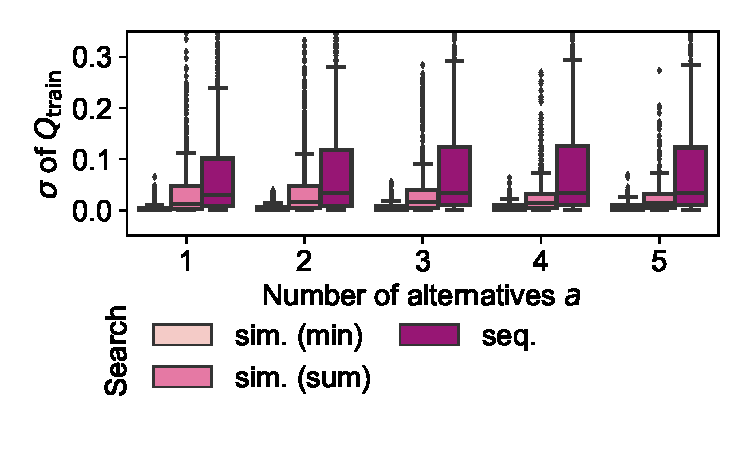
\includegraphics[width=\textwidth, trim=15 20 10 10, clip]{plots/afs-impact-search-stddev-train-objective.pdf}
		\caption{Training-set objective value.}
		\label{fig:afs:impact-search-stddev-train-objective}
	\end{subfigure}
	\hfill
	\begin{subfigure}[t]{0.49\textwidth}
		\centering
		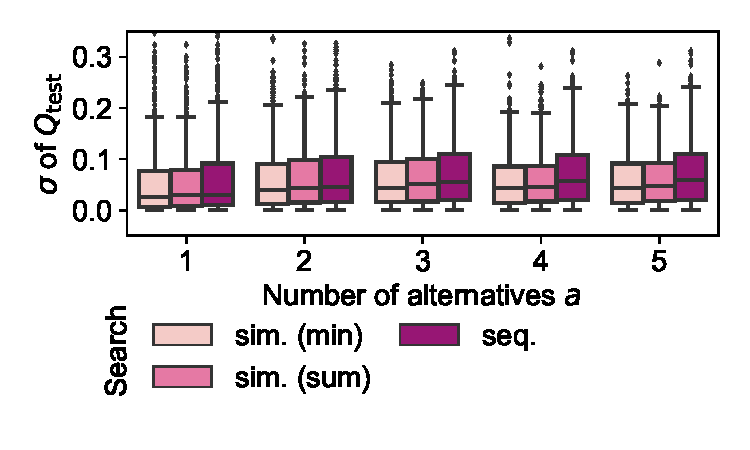
\includegraphics[width=\textwidth, trim=15 20 10 10, clip]{plots/afs-impact-search-stddev-test-objective.pdf}
		\caption{Test-set objective value.}
		\label{fig:afs:impact-search-stddev-test-objective}
	\end{subfigure}
	\caption{
		Standard deviation of feature-set quality within search runs over the number of alternatives~$a$, by search method for alternatives and evaluation metric.
		Results with \emph{MI} as feature-selection method and $k=5$.
		Y-axes are truncated to improve readability.
	}
	\label{fig:afs:impact-search-stddev}
\end{figure*}

\paragraph{Variance in feature-set quality}

As expected, the search method influences how much the training-set objective value~$Q$ varies among alternatives within each search run.
Figure~\ref{fig:afs:impact-search-stddev-train-objective} visualizes this observation for \emph{MI}, though it applies to all other white-box feature-selection methods as well.
Each box in the figure shows how the variance within individual search runs for alternatives is distributed over other experimental settings, e.g., datasets and cross-validation folds.
In particular, the quality of multiple alternatives from the same search run varies less for simultaneous than sequential search and less for min-aggregation than sum-aggregation.
However, this difference in variance largely disappears on the test set, for the objective value (Figure~\ref{fig:afs:impact-search-stddev-test-objective}) as well as prediction performance.
This effect might result from overfitting:
Even with similar training-set quality, some alternatives may generalize better than others.
Thus, the variance in test feature-set quality caused by overfitting could alleviate the effect on variance caused by the search method.

\begin{figure*}[t]
	\centering
	\begin{subfigure}[t]{0.49\textwidth}
		\centering
		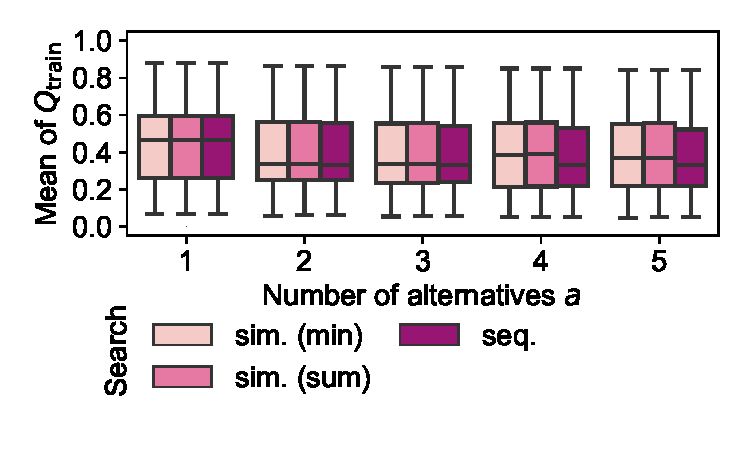
\includegraphics[width=\textwidth, trim=15 20 10 10, clip]{plots/afs-impact-search-mean-train-objective.pdf}
		\caption{Training-set objective value.}
		\label{fig:afs:impact-search-mean-train-objective}
	\end{subfigure}
	\hfill
	\begin{subfigure}[t]{0.49\textwidth}
		\centering
		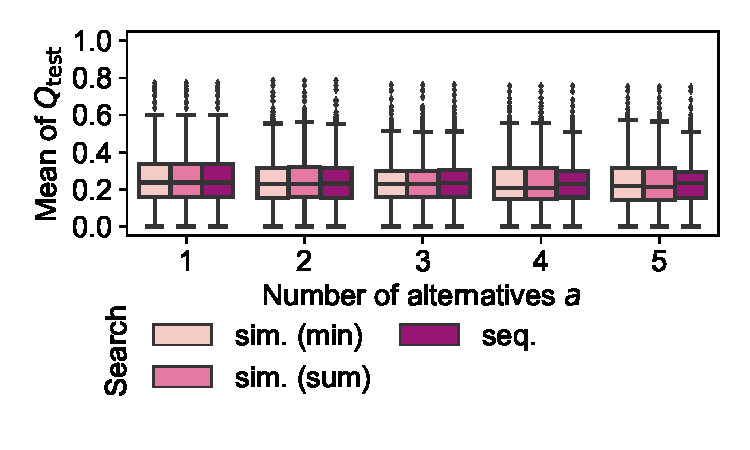
\includegraphics[width=\textwidth, trim=15 20 10 10, clip]{plots/afs-impact-search-mean-test-objective.pdf}
		\caption{Test-set objective value.}
		\label{fig:afs:impact-search-mean-test-objective}
	\end{subfigure}
	\caption{
		Mean of feature-set quality within search runs over the number of alternatives~$a$, by search method for alternatives and evaluation metric.
		Results with \emph{MI} as feature-selection method and $k=5$.
	}
	\label{fig:afs:impact-search-mean}
\end{figure*}

\paragraph{Average value of feature-set quality}

While obtaining quality-homogeneous alternatives can be one goal of simultaneous search, the main selling point would be obtaining alternatives of higher average quality than sequential search.
However, this potential advantage rarely materialized in our experiments.
In particular, Figure~\ref{fig:afs:impact-search-mean-train-objective} compares the distribution of the mean training-set objective in search runs for \emph{MI} as the feature-selection method.
We observe that all three search methods yield similar distributions of training-set objective values.
This observation holds for feature-set quality on the test set (Figure~\ref{fig:afs:impact-search-mean-test-objective}) as well.
Further, the other four feature-selection methods besides \emph{MI} also do not show a general quality advantage of simultaneous search.
Finally, depending on the concrete experimental setting, either sequential or simultaneous search can yield significantly higher quality than the other search method, even if the overall mean difference is close to zero.

\begin{table*}[t]
	\centering
	\caption{
		Frequency of optimization statuses (Section~\ref{sec:afs:experimental-design:evaluation}) by feature-selection method and search method for alternatives.
		Results with $k=5$, $a \in \{1,2,3,4,5\}$, and excluding \emph{Greedy Wrapper}, which uses the solver for satisfiability checking rather than optimizing.
		Each row adds up to 100\%.
	}
	\begin{tabular}{llrrr}
		\toprule
		\multirow{2}{*}{Feature selection} & \multirow{2}{*}{Search} & \multicolumn{3}{c}{Optimization status} \\
		\cmidrule(r){3-5}
		& & Infeasible & Feasible & Optimal \\
		\midrule
		FCBF & seq. & 74.51\% & 0.00\% & 25.49\% \\
		FCBF & sim. (min) & 73.07\% & 1.73\% & 25.20\% \\
		FCBF & sim. (sum) & 73.07\% & 2.19\% & 24.75\% \\
		MI & seq. & 4.93\% & 0.00\% & 95.07\% \\
		MI & sim. (min) & 4.67\% & 9.60\% & 85.73\% \\
		MI & sim. (sum) & 4.67\% & 3.17\% & 92.16\% \\
		Model Gain & seq. & 4.93\% & 0.00\% & 95.07\% \\
		Model Gain & sim. (min) & 4.67\% & 5.55\% & 89.79\% \\
		Model Gain & sim. (sum) & 4.67\% & 1.92\% & 93.41\% \\
		mRMR & seq. & 4.88\% & 9.63\% & 85.49\% \\
		mRMR & sim. (min) & 4.67\% & 49.04\% & 46.29\% \\
		mRMR & sim. (sum) & 4.67\% & 67.39\% & 27.95\% \\
		\bottomrule
	\end{tabular}
	\label{tab:afs:impact-search-fs-method-optimization-status}
\end{table*}

\paragraph{Optimization status}

One reason why simultaneous search fails to consistently beat the quality of sequential search is that search results may be suboptimal.
For \emph{Greedy Wrapper}, the search is heuristic per se and does not cover the entire search space.
For all feature-selection methods, the solver can time out.
In particular, the corresponding solver status \emph{feasible} occurs more often for simultaneous than sequential search, as Table~\ref{tab:afs:impact-search-fs-method-optimization-status} shows.
Such timeout-affected simultaneous solutions can be worse than optimal sequential solutions.
The optimization status \emph{not solved}, i.e., not finding a feasible solution without proving infeasibility, did not occur in the displayed results.
The feature-selection method \emph{mRMR} is especially prone to suboptimal solutions, likely because it has a more complex objective than~\emph{MI} and \emph{Model Gain}.
In contrast, \emph{FCBF} often results in infeasible optimization problems since its constraints preventing the selection of redundant features might prevent finding any valid feature set of size~$k$.

Further, the fraction of timeouts strongly depends on the number of alternatives~$a$.
E.g., for simultaneous search with $k=5$ and sum-aggregation, roughly 8\% of the white-box searches timed out for one alternative but 20\% for three alternatives and 30\% for five alternatives.
While we grant simultaneous searches proportionally more time to obtain more feature sets, the runtime increases clearly super-proportionally, as we analyze next.

\begin{table}[t]
	\centering
	\caption{
		Mean optimization time by feature-selection method and search method for alternatives.
		Results with $k=5$ and $a \in \{1,2,3,4,5\}$.
	}
	\begin{tabular}{lrrr}
		\toprule
		\multirow{2}{*}{Feature selection} & \multicolumn{3}{c}{Optimization time} \\
		\cmidrule(r){2-4}
		& Seq. & Sim. (min) & Sim. (sum) \\
		\midrule
		FCBF & 0.22~s & 11.91~s & 13.09~s \\
		Greedy Wrapper & 54.23~s & 61.10~s & 63.45~s \\
		MI & 0.03~s & 48.25~s & 25.39~s \\
		Model Gain & 0.03~s & 30.91~s & 19.98~s \\
		mRMR & 34.12~s & 157.87~s & 189.76~s \\
		\bottomrule
	\end{tabular}
	\label{tab:afs:impact-search-fs-method-optimization-time}
\end{table}

\paragraph{Optimization time}

The optimization time also favors sequential search.
As Table~\ref{tab:afs:impact-search-fs-method-optimization-time} shows, the mean optimization time of sequential search is lower for all five feature-selection methods, partly by orders of magnitude.
Further, \emph{FCBF}, \emph{MI}, and \emph{Model Gain} experience a dramatic increase in optimization time with parameter~$a$.
E.g., for simultaneous search with $k=5$ and sum-aggregation, \emph{MI} has a mean optimization time of 0.03~s for $a=1$, 0.09~s for $a=2$, 0.31~$s$ for $a=3$, 3.84~$s$ for $a=4$, and 122.69~s for $a=5$.
In contrast, the runtime increase is considerably less for sequential search, which shows an approximately linear trend with the number of alternatives.

Another interesting question is how the runtime relates to~$n$, the number of features in the dataset.
Our experimental data show a positive correlation, as we expected.
However, the observed trend is very noisy, particularly for simultaneous search.
E.g., runtimes vary considerably even for a fixed~$n$, and some higher-dimensional datasets even show lower average runtimes than lower-dimensional ones.
This result indicates that other factors than~$n$ influence runtime.
Besides factors related to the datasets and experimental design, the heuristics used by the solver may also cause the runtime to fluctuate considerably.

Based on all results described in this section, we focus on sequential search in the following, and we also recommend it to users.
In particular, it was significantly faster than simultaneous search while yielding similar feature-set quality.

\subsection{User Parameters \texorpdfstring{$a$ And $\tau$}{}} % \texorpdfstring prevents warning "Token not allowed in a PDF string"
\label{sec:afs:evaluation:parameters}

\begin{figure*}[t]
	\begin{subfigure}[t]{0.49\textwidth}
		\centering
		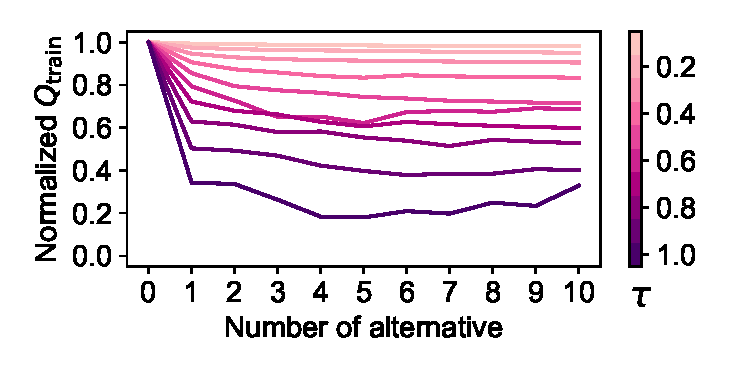
\includegraphics[width=\textwidth, trim=15 15 20 10, clip]{plots/afs-impact-num-alternatives-tau-train-objective-max.pdf}
		\caption{
			Training-set objective value.
			Infeasible feature sets excluded.
		}
		\label{fig:afs:impact-num-alternatives-tau-train-objective-max}
	\end{subfigure}
	\hfill
	\begin{subfigure}[t]{0.49\textwidth}
		\centering
		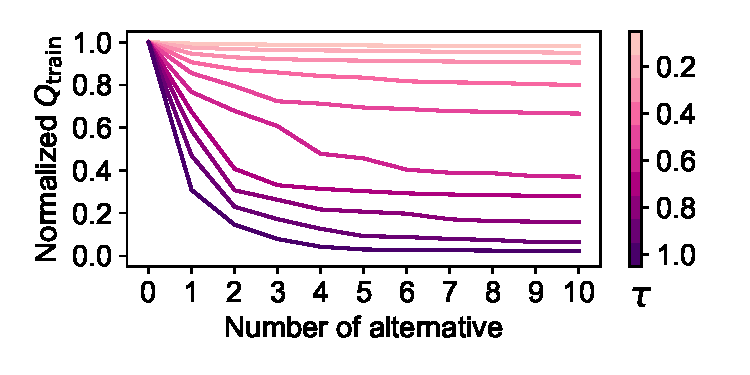
\includegraphics[width=\textwidth, trim=15 15 20 10, clip]{plots/afs-impact-num-alternatives-tau-train-objective-max-fillna.pdf}
		\caption{
			Training-set objective value.
			Infeasible feature sets assigned a quality of~0.
		}
		\label{fig:afs:impact-num-alternatives-tau-train-objective-max-fillna}
	\end{subfigure}
	\\
	\begin{subfigure}[t]{0.49\textwidth}
		\centering
		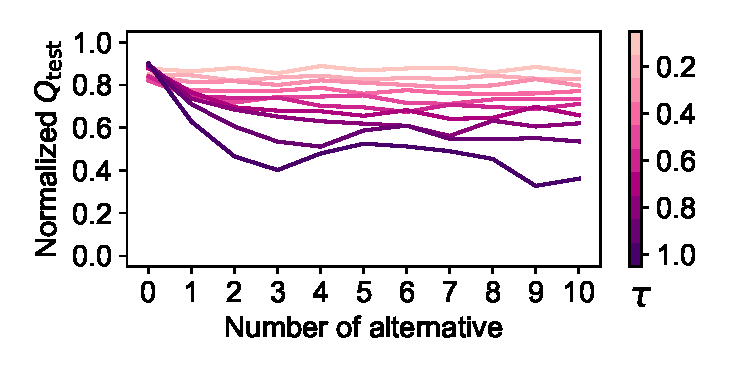
\includegraphics[width=\textwidth, trim=15 15 20 10, clip]{plots/afs-impact-num-alternatives-tau-test-objective-max.pdf}
		\caption{
			Test-set objective value.
			Infeasible feature sets excluded.
		}
		\label{fig:afs:impact-num-alternatives-tau-test-objective-max}
	\end{subfigure}
	\hfill
	\begin{subfigure}[t]{0.49\textwidth}
		\centering
		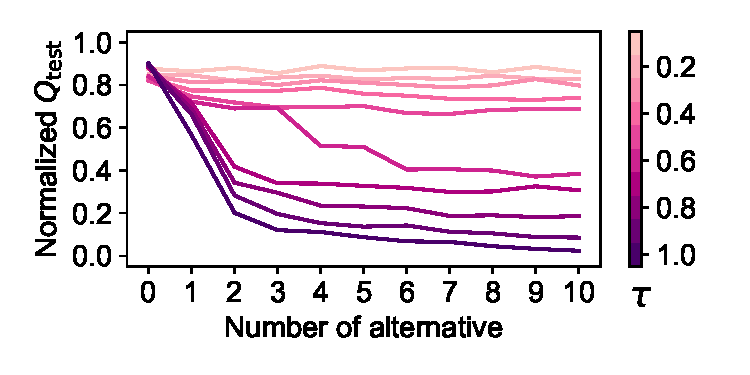
\includegraphics[width=\textwidth, trim=15 15 20 10, clip]{plots/afs-impact-num-alternatives-tau-test-objective-max-fillna.pdf}
		\caption{
			Test-set objective value.
			Infeasible feature sets assigned a quality of~0.
		}
		\label{fig:afs:impact-num-alternatives-tau-test-objective-max-fillna}
	\end{subfigure}
	\\
	\begin{subfigure}[t]{0.49\textwidth}
		\centering
		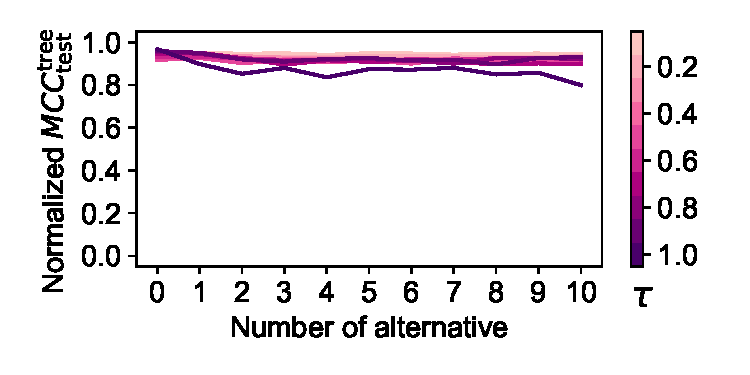
\includegraphics[width=\textwidth, trim=15 15 20 10, clip]{plots/afs-impact-num-alternatives-tau-decision-tree-test-mcc-max.pdf}
		\caption{
			Test-set prediction performance.
			Infeasible feature sets excluded.
		}
		\label{fig:afs:impact-num-alternatives-tau-decision-tree-test-mcc-max}
	\end{subfigure}
	\hfill
	\begin{subfigure}[t]{0.49\textwidth}
		\centering
		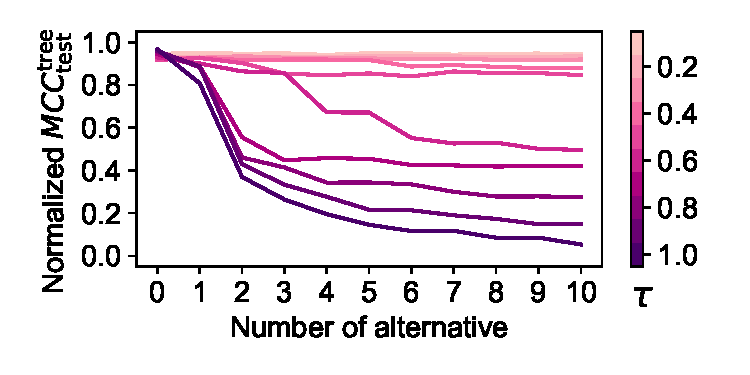
\includegraphics[width=\textwidth, trim=15 15 20 10, clip]{plots/afs-impact-num-alternatives-tau-decision-tree-test-mcc-max-fillna.pdf}
		\caption{
			Test-set prediction performance.
			Infeasible feature sets assigned a quality of~0.
		}
		\label{fig:afs:impact-num-alternatives-tau-decision-tree-test-mcc-max-fillna}
	\end{subfigure}
	\caption{
		Mean of feature-set quality, max-normalized per search run for alternatives, over the number of alternatives and dissimilarity threshold~$\tau$, by evaluation metric.
		Results from sequential search with \emph{MI} as feature-selection method and $k=10$.
	}
	\label{fig:afs:impact-num-alternatives-tau-quality}
\end{figure*}

\paragraph{Feature-set quality}

One would expect a decrease in feature-set quality with an increasing number of alternatives~$a$ and dissimilarity threshold~$\tau$, giving users control over alternatives.
In particular, higher values of the two user parameters introduce more (for~$a$) and stronger (for~$\tau$) constraints to the optimization problem.
Figure~\ref{fig:afs:impact-num-alternatives-tau-quality} shows this decreasing quality trend for \emph{MI}-based feature selection.
Since feature-set quality varies significantly among datasets, we display it normalized to $[0,1]$ within each search run for alternatives:
We shift the range of all evaluation metrics to~$[0,1]$ and max-normalize feature-set quality for each search of alternatives, i.e., the highest feature-set quality in the search run is set to~1, and the other qualities are scaled accordingly.

As visible in Figure~\ref{fig:afs:impact-num-alternatives-tau-quality}, there might be multiple alternatives of similar quality, particularly for low values of~$\tau$.
Further, the objective value decreases most from the original, unconstrained feature set, i.e., the zeroth alternative in the figures, to the first alternative, but the decrease is less beyond.
Note that Figure~\ref{fig:afs:impact-num-alternatives-tau-quality} averages the normalized feature-set quality over datasets with different dimensionality.
In our experiments, datasets with more features~$n$ tend to experience a smaller decrease in quality over~$a$ and~$\tau$.
As higher-dimensional datasets offer more options for alternatives, this observation makes sense.
However, this effect is not guaranteed since datasets with many features could also contain many useless features instead of interesting alternatives.

The overall decrease in quality is slightly less pronounced for the test-set objective value (Figure~\ref{fig:afs:impact-num-alternatives-tau-test-objective-max}) than for the training-set one (Figure~\ref{fig:afs:impact-num-alternatives-tau-train-objective-max}) since overfitting might occur.
In particular, the original feature set can even have lower test-set quality than the subsequent alternatives.
The change in feature-set quality becomes even less clear when using the alternative feature sets to train prediction models, i.e., decision trees.
As Figure~\ref{fig:afs:impact-num-alternatives-tau-decision-tree-test-mcc-max} shows, the prediction performance varies little over the number of alternatives and the dissimilarity threshold~$\tau$.
In particular, the optimization objective~$Q$ may only partially indicate actual prediction performance since the former may use a simplified feature-set quality criterion.
Indeed, the overall correlation between optimization objective~$Q$ and prediction MCC is only weak to moderate in our experiments.
Among the feature-selection methods, this correlation is highest for \emph{Greedy Wrapper} but also not perfect there.
In particular, the search procedure of \emph{Greedy Wrapper} evaluates feature sets with a validation split of the training set.
MCC on this holdout set may not perfectly correspond to MCC on the test set, which is not used in the search.

\begin{figure}[t]
	\centering
	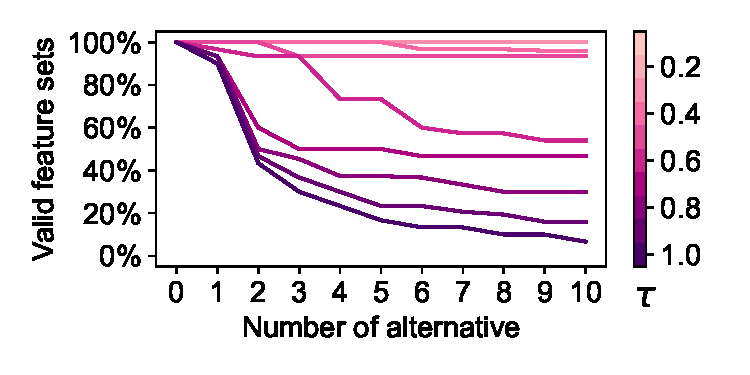
\includegraphics[width=\columnwidth, trim=15 15 20 10, clip]{plots/afs-impact-num-alternatives-tau-optimization-status.pdf}
	\caption{
		Fraction of optimization runs yielding a valid feature set over the number of alternatives and dissimilarity threshold~$\tau$.
		Results from sequential search with \emph{MI} as feature-selection method and $k=10$.
	}
	\label{fig:afs:impact-num-alternatives-tau-optimization-status}
\end{figure}

\paragraph{Optimization status}

Increasing~$a$ and~$\tau$ does not only affect quality but can also render the optimization problem infeasible, i.e., no valid alternative might exist.
Figure~\ref{fig:afs:impact-num-alternatives-tau-optimization-status} visualizes how the percentage of valid feature sets develops over~$a$ and~$\tau$ in our experiments.
In our prior analysis of feature-set quality, we excluded infeasible feature sets.
For comparison, Figures~\ref{fig:afs:impact-num-alternatives-tau-train-objective-max-fillna}, \ref{fig:afs:impact-num-alternatives-tau-test-objective-max-fillna}, and~\ref{fig:afs:impact-num-alternatives-tau-decision-tree-test-mcc-max-fillna} show the same data as Figures~\ref{fig:afs:impact-num-alternatives-tau-train-objective-max}, \ref{fig:afs:impact-num-alternatives-tau-test-objective-max}, and~\ref{fig:afs:impact-num-alternatives-tau-decision-tree-test-mcc-max} but with the quality of infeasible feature sets set to zero, i.e., the theoretical minimum quality after we shifted the value ranges of evaluation metrics.
In these three figures, the decrease in feature-set quality is noticeably stronger for all evaluation metrics.
In particular, test-set prediction performance, which is relatively stable when excluding infeasible feature sets (Figure~\ref{fig:afs:impact-num-alternatives-tau-decision-tree-test-mcc-max}), also decreases now (Figure~\ref{fig:afs:impact-num-alternatives-tau-decision-tree-test-mcc-max-fillna}).

In contrast, if only considering valid feature sets, the mean quality may even increase over the number of alternatives, as visible in Figure~\ref{fig:afs:impact-num-alternatives-tau-train-objective-max} and Figure~\ref{fig:afs:impact-num-alternatives-tau-test-objective-max} for $\tau=1.0$.
This counterintuitive phenomenon can occur because some datasets run out of valid feature sets sooner than others, so the average quality may be determined for different sets of datasets at each number of alternatives.

\begin{figure*}[t]
	\centering
	\begin{subfigure}[t]{0.49\textwidth}
		\centering
		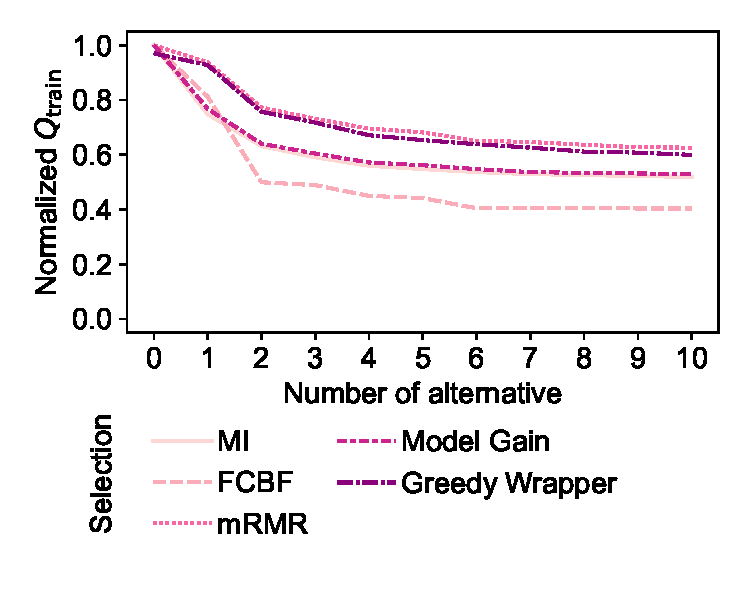
\includegraphics[width=\textwidth, trim=15 30 10 10, clip]{plots/afs-impact-num-alternatives-fs-method-train-objective-max-fillna.pdf}
		\caption{
			Over the number of alternatives~$a$.
		}
		\label{fig:afs:impact-num-alternatives-fs-method-train-objective-max-fillna}
	\end{subfigure}
	\hfill
	\begin{subfigure}[t]{0.49\textwidth}
		\centering
		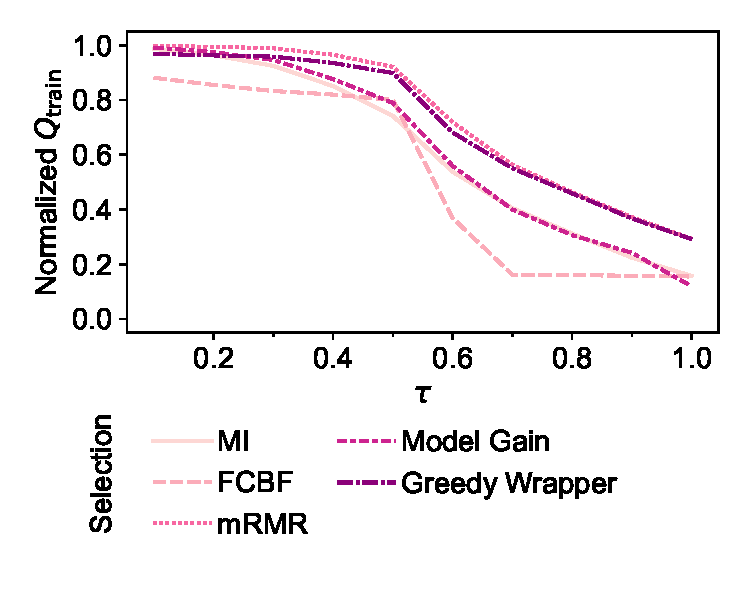
\includegraphics[width=\textwidth, trim=15 30 10 10, clip]{plots/afs-impact-tau-fs-method-train-objective-max-fillna.pdf}
		\caption{
			Over the dissimilarity threshold~$\tau$.
		}
		\label{fig:afs:impact-tau-fs-method-train-objective-max-fillna}
	\end{subfigure}
	\caption{
		Mean of training-set objective value, max-normalized per search run for alternatives, by feature-selection method and evaluation metric.
		Infeasible feature sets assigned a quality of~0.
		Results from sequential search with $k=10$.
	}
	\label{fig:afs:impact-parameters-fs-method}
\end{figure*}

\paragraph{Influence of feature-selection method}

While we discussed \emph{MI} before, the decrease in the objective value over parameter~$a$ occurs for all feature-selection methods in our experiments, as Figure~\ref{fig:afs:impact-num-alternatives-fs-method-train-objective-max-fillna} shows.
However, the strength of the decrease varies considerably among the feature-selection methods.
For example, \emph{Greedy Wrapper} and \emph{mRMR} show the least effect of~$a$.
The effect of~$\tau$ also depends on the feature-selection method, as Figure~\ref{fig:afs:impact-tau-fs-method-train-objective-max-fillna} shows.
Again, \emph{MI} and \emph{Model Gain}, which both use the simple univariate objective (Equation~\ref{eq:afs:univariate-filter}), show a stronger trend than \emph{Greedy Wrapper} and \emph{mRMR}.
The fifth feature-selection method, \emph{FCBF}, also exhibits a clear quality decrease over~$a$ and~$\tau$, mainly due to a high rate of infeasible feature sets rather than a quality decrease of the found feature sets.
Ultimately, choosing a particular feature-selection method depends on the use case.
Thereby, users should be aware that effects regarding alternative feature sets may depend on this choice.

\section{Related Work}
\label{sec:afs:related-work}

In this section, we review related work from the field of feature selection and other areas relevant to this article.
To our knowledge, searching for optimal alternative feature sets in the sense of this article is novel.
However, there is literature on optimal alternatives outside the field of feature selection.
Additionally, there has been research focused on discovering multiple diverse feature sets.

\paragraph{Feature selection}

% Traditional + ensemble feature selection
Most feature-selection methods yield one solution~\cite{borboudakis2021extending}, though there are some exceptions~\cite{emmanouilidis1999selecting, mueller2021feature, siddiqi2020genetic}, e.g., fostering diversity within wrapper methods.
Ensemble feature selection~\cite{saeys2008robust, seijo2017ensemble} combines feature-selection results obtained by different feature-selection methods or on different samples of the data.
There, diversity can be an auxiliary goal to improve prediction performance~\cite{guru2018alternative, liu2019subspace, woznica2012model}.
In addition, the notion of feature-set diversity differs from ours.
In particular, these approaches give users less control over alternatives, e.g., do not enforce alternatives with hard constraints.

% Statistically equivalent feature sets
Approaches for statistically equivalent feature sets~\cite{borboudakis2021extending, lagani2017feature} use statistical tests to determine feature sets that are equivalent for predictions.
In contrast, we do not require equivalent quality but allow users to control the number and dissimilarity of alternatives directly.

% Constrained feature selection
There also is work on constraints for feature selection, e.g., for feature cost~\cite{paclik2002feature}, feature groups~\cite{yuan2006model}, or domain knowledge~\cite{bach2022empirical, groves2015toward}.
Such constraints do not explicitly target alternatives but could be integrated into our integer-programming formulation as well.

\paragraph{Subgroup discovery}

Diversity also is an issue in subgroup set discovery, which searches for interesting regions in the data space instead of selecting features as a whole.
\cite{leeuwen2012diverse} presents six strategies to facilitate subgroup diversity. 
Two are directly transferable to feature selection, but the criteria for being alternative are different from ours.
In particular, one strategy prunes similar subgroups with exactly the same quality as previous solutions. 
The other one limits the number of subgroups a feature may occur in but does not constrain the overlap of subgroups per se.

\paragraph{Clustering}

Finding alternative solutions has been addressed extensively in the field of clustering.
\cite{bailey2014alternative} gives a taxonomy and describes algorithms for alternative clustering.
Our problem definition is different in several respects.
The notion of dissimilarity differs since we strive for differently composed feature sets, while alternative clustering targets different assignments of data objects to clusters.
Next, using constraints is only one approach to obtain alternative clusterings.
Finally, we optimize feature-set quality in a supervised prediction scenario while clustering is unsupervised.

\paragraph{Subspace search}

Finding several useful feature sets also is part of subspace clustering~\cite{hu2018subspace, mueller2009relevant} and subspace search~\cite{fouche2021efficient, nguyen20134s, trittenbach2019dimension}.
These approaches strive to improve data-mining algorithms by using subspaces, i.e., feature sets, and not all features.
Some approaches explicitly try to remove redundancy between subspaces~\cite{mueller2009relevant, nguyen20134s} or increase subspace diversity~\cite{fouche2021efficient, trittenbach2019dimension}.
See \cite{hu2018subspace} for an overview.
Alternative feature selection is different in at least one of the following aspects:
First, the objective function, i.e., the notion of quality, differs.
Second, definitions of subspace redundancy may hinge on feature values instead of binary selection decisions.
Third, users typically do not have any control over the dissimilarity. 
At best, there is a regularization parameter rather than a hard threshold.

\paragraph{Explainable artificial intelligence (XAI)}

In XAI, alternative explanations might provide additional insights, allow to test different hypotheses, and foster trust in the predictions~\cite{kim2021multi, wang2019designing}.
In contrast, obtaining significantly different explanations for a prediction might raise doubts regarding their meaningfulness \cite{jain2019attention}.
Diversity is a criterion studied for various explainers, e.g., for counterfactuals~\cite{dandl2020multi, karimi2020model, mohammadi2021scaling, mothilal2020explaining, russell2019efficient, wachter2017counterfactual}, criticisms~\cite{kim2016examples}, or semifactual explanations~\cite{artelt2022even}.
There are several approaches to foster diversity, e.g., ensembling explanations~\cite{silva2019produce}, considering multiple local minima~\cite{wachter2017counterfactual}, using a search algorithm that maintains diversity~\cite{dandl2020multi}, extending the optimization objective~\cite{artelt2022even, kim2016examples, mothilal2020explaining}, or introducing constraints~\cite{karimi2020model, mohammadi2021scaling, russell2019efficient}.
The last option is similar to the way we enforce alternatives.
Of all these approaches, only~\cite{artelt2022even, mohammadi2021scaling, mothilal2020explaining} introduce parameters to control the diversity of solutions; only~\cite{mohammadi2021scaling} offers a user-friendly dissimilarity threshold in~$[0,1]$, while the other two approaches regularize the objective.
Further, all the previously mentioned XAI techniques provide local explanations, i.e., aim at prediction outcomes for individual data objects rather than optimizing the global prediction quality of feature sets.

\paragraph{Rashomon sets}

A Rashomon set is a set of prediction models that reach a certain, e.g., close-to-optimal, prediction performance~\cite{fisher2019all}.
Despite similar performance, these models may still assign different feature importance scores, leading to different explanations~\cite{laberge2023partial}.
Thus, Rashomon sets may yield partial information about alternative feature sets.
However, approaches for Rashomon sets do not explicitly search for alternative feature sets as a whole, i.e., feature sets satisfying a dissimilarity threshold relative to other sets.
Instead, these approaches focus on the range of each feature's importance over prediction models.
Further, our notion of alternatives is not bound to model-based feature importance but encompasses a broader range of feature-selection methods.
Finally, we use importance scores from one model instead of multiple models to find importance-based alternatives.

\section{Conclusions and Future Work}
\label{sec:afs:conclusion}

\paragraph{Conclusions}

Our article has studied alternative feature selection, the problem of identifying diverse feature sets that simultaneously maintain high quality. 
We formalized alternative feature selection as an optimization problem, using constraints that are independent of the chosen feature-selection method. 
These constraints can be combined with other constraints on feature sets and offer users control over diversity via two parameters: the number of alternatives and a dissimilarity threshold.
We analyzed the computational complexity of this optimization problem, showing its $\mathcal{NP}$-hardness. 
Additionally, we discussed the integration of various categories of feature-selection methods. 
Finally, we assessed the effectiveness of alternative feature selection using 30 datasets representing binary-classification problems.

\paragraph{Future work}

In the current article, we conducted a broad quantitative evaluation of alternative feature selection on datasets from various domains.
Practitioners can employ alternative feature selection in domain-specific case studies and evaluate the alternative feature sets qualitatively, thereby assessing their usefulness for interpretability.
Within alternative feature selection, opportunities exist to modify the formulation of the optimization problem, such as by incorporating soft constraints or adopting a multi-objective optimization approach instead of employing hard constraints. 
Furthermore, one can integrate additional feature-selection methods into the search for alternatives, including embedded methods. 
Finally, there is potential for enhancing the efficiency of the search for alternatives, particularly in the case of simultaneous search, by developing heuristics instead of seeking exact solutions to the optimization problem.

\backmatter

\section*{Declarations}

\bmhead{Funding}

This work was supported by the Ministry of Science, Research and the Arts Baden-W\"urttemberg, project \emph{Algorithm Engineering for the Scalability Challenge (AESC)}.
%TODO: check with Prof. Böhm if this still is the appropriate funding declaration (copied from arXiv version)

\bmhead{Conflict of interest}

On behalf of all authors, the corresponding author states that there is no conflict of interest.

\bmhead{Availability of data and materials}

All experimental data are available online at \url{https://doi.org/10.35097/1975}.

\bmhead{Code availability}

The code is available online at \url{https://github.com/Jakob-Bach/Alternative-Feature-Selection}.

\begin{appendices}

\section{Appendix}
\label{sec:afs:appendix}

In this section, we provide technical details and proofs.
Section~\ref{sec:afs:appendix:simultaneous-objective-aggregation} discusses aggregation operators for the objective of simultaneous search (Equation~\ref{eq:afs:afs-simultaneous}).
Section~\ref{sec:afs:appendix:univariate-complete-optimization-problem} contains complete definitions of the alternative-feature-selection problem (Section~\ref{sec:afs:approach:constraints}) for the univariate objective (Equation~\ref{eq:afs:univariate-filter}).
Section~\ref{sec:afs:appendix:complexity-proofs} supplies proofs for the complexity analysis (Section~\ref{sec:afs:approach:complexity}).

\subsection{Aggregation Operators for Simultaneous Search}
\label{sec:afs:appendix:simultaneous-objective-aggregation}

In this section, we discuss operators to aggregate the feature-set quality of multiple alternatives in the objective of simultaneous search (Equation~\ref{eq:afs:afs-simultaneous}).

\paragraph{Sum-aggregation}

The arguably simplest way to aggregate the qualities of multiple feature sets is to sum them up, which we call \emph{sum-aggregation}, as defined by Equation~\ref{eq:afs:afs-simultaneous-sum-objective}:
%
\begin{equation}
	\max_{s^{(0)}, \dots, s^{(a)}} \sum_{i=0}^a Q(s^{(i)},X,y)
	\label{eq:afs:afs-simultaneous-sum-objective}
\end{equation}
%
While this objective fosters a high average quality of feature sets, it does not guarantee that the alternatives have similar quality:
%
\begin{example}[Sum-aggregation]
	Consider $n=6$~features with univariate feature qualities (Equation~\ref{eq:afs:univariate-filter}) $q = (9,8,7,3,2,1)$, feature-set size~$k=3$, number of alternatives~$a=2$, and dissimilarity threshold~$\tau = 0.5$, which permits an overlap of one feature between sets here.
	Sequential search yields the selection $s^{(0)} = (1,1,1,0,0,0)$, $s^{(1)} = (1,0,0,1,1,0)$, and $s^{(2)} = (0,1,0,1,0,1)$, with a summed quality of $24+14+12=50$.
	One possible simultaneous-search solution consists of the feature sets $s^{(0)} = (1,1,0,1,0,0)$, $s^{(1)} = (1,0,1,0,1,0)$, and $s^{(2)} = (0,1,1,0,0,1)$, with a summed quality of $20+18+16=54$.
	Another possible simultaneous-search solution is $s^{(0)} = (1,1,0,0,0,1)$, $s^{(1)} = (1,0,1,0,1,0)$, and $s^{(2)} = (0,1,1,1,0,0)$, with a summed quality of $18+18+18=54$.
	\label{ex:afs:sum-aggregation}
\end{example}
%
This example allows several insights.
First, sequential search yields worse quality than simultaneous search here, i.e., 50 vs.~54.
Second, the feature-set qualities of the sequential solution, i.e., 24, 14, and~12, differ significantly.
Third, simultaneous search can yield multiple solutions whose feature-set quality is differently balanced.
Here, the feature-set qualities in the second simultaneous-search solution, i.e., 18, 18, and~18, are more balanced than in the first, i.e., 20, 18, and~16.
However, both solutions are equally optimal for sum-aggregation.

\paragraph{Min-aggregation}

To actively foster balanced feature-set qualities in simultaneous search, we propose \emph{min-aggregation} in the objective, as defined by Equation~\ref{eq:afs:afs-simultaneous-min-objective}:
%
\begin{equation}
	\max_{s^{(0)}, \dots, s^{(a)}} \min_{i \in \{0, \dots, a\}} Q(s^{(i)},X,y) \\
	\label{eq:afs:afs-simultaneous-min-objective}
\end{equation}
%
In the terminology of social choice theory, this objective uses an egalitarian rule instead of a utilitarian one~\cite{myerson1981utilitarianism}.
In particular, \emph{min-aggregation} maximizes the quality of the worst selected alternative.
Thereby, it incentivizes all alternatives to have high quality and implicitly balances their quality.

Note that optimizing the objective with either sum-aggregation or min-aggregation does not necessarily optimize the other.
We already showed a solution optimizing sum-aggregation but not min-aggregation (Example~\ref{ex:afs:sum-aggregation}).
In the following, we demonstrate the other direction:
%
\begin{example}[Min-aggregation]
	Consider $n=6$~features with univariate feature qualities (Equation~\ref{eq:afs:univariate-filter}) $q = (11,10,6,5,4,1)$, feature-set size~$k=3$, number of alternatives~$a=1$, and dissimilarity threshold~$\tau = 0.5$, which permits an overlap of one feature between sets here.
	One solution optimizing the objective with min-aggregation is $s^{(0)} = (1,1,0,0,1,0)$ and $s^{(1)} = (1,0,1,1,0,0)$, with a summed quality of $25+22=47$.
	Another solution is $s^{(0)} = (1,1,0,0,0,1)$ and $s^{(1)} = (1,0,1,1,0,0)$, with a summed quality of $22+22=44$.
	\label{ex:afs:min-aggregation}
\end{example}
%
While both solutions have the same minimum feature-set quality, only the first solution optimizes the objective with sum-aggregation.
In particular, min-aggregation permits reducing the quality of feature sets as long as it remains above the minimum of all sets.

From the technical perspective, Equation~\ref{eq:afs:afs-simultaneous-min-objective} has the disadvantage of being non-linear regarding the decision variables $s^{(0)}, \dots, s^{(a)}$.
However, we can linearize it with one constraint per feature set and an auxiliary variable~$Q_{\text{min}}$, as shown in Equation~\ref{eq:afs:afs-simultaneous-min-objective-linear}:
%
\begin{equation}
	\begin{gathered}
		\max_{s^{(0)}, \dots, s^{(a)}} \quad Q_{\text{min}} \\
		\begin{aligned}
			\text{s.t.:}~\forall i \in \{0, \dots, a\}:~Q_{\text{min}} &\leq Q(s^{(i)},X,y) \\
			Q_{\text{min}} &\in \mathbb{R}
		\end{aligned}
	\end{gathered}
	\label{eq:afs:afs-simultaneous-min-objective-linear}
\end{equation}
%
As we maximize~$Q_{\text{min}}$, this variable will implicitly assume the actual minimum value of~$Q(s^{(i)},X,y)$ with equality since the solution would not be optimal otherwise.
This situation relieves us from introducing further auxiliary variables that are usually necessary when linearizing maximum or minimum expressions~\cite{mosek2022modeling}.

\paragraph{Further approaches for balancing quality}

Min-aggregation provides no control or guarantee of how much the feature-set qualities will actually differ between alternatives since it only incentivizes high quality for all sets.
One can alleviate this issue by adapting the objective or constraints.
First, related work on \textsc{Multi-Way Number Partitioning} (Section~\ref{sec:afs:approach:complexity:uni}) also uses other objectives for balancing~\cite{korf2010objective, lawrinenko2017identical}.
E.g., one could minimize the difference between maximum and minimum feature-set quality.
Second, one could use sum-aggregation but constrain the minimum or maximum quality of sets, or the difference between the qualities.
However, such constraint-based approaches introduce one or several parameters bounding feature-set quality, which are difficult to determine a priori.
Third, one could treat balancing qualities as another objective besides maximizing the summed quality.
One can then optimize two objectives simultaneously, filtering results for Pareto-optimal solutions or optimizing a weighted combination of the two objectives.
In both cases, users may need to define an acceptable trade-off between the objectives.
It is an open question if a solution always exists that jointly optimizes min- and sum-aggregation.
If yes, then optimizing a weighted combination of the two objectives would also optimize each of them on its own, assuming positive weights.

\subsection{Complete Specifications of the Optimization Problem for the Univariate Objective}
\label{sec:afs:appendix:univariate-complete-optimization-problem}

In this section, we provide complete specifications of the alternative-feature-selection problem for sequential and simultaneous search.
In particular, we combine all relevant definitions and equations from Section~\ref{sec:afs:approach}.
We use the objective of univariate filter feature selection (Equation~\ref{eq:afs:univariate-filter}).
The corresponding feature qualities $q(\cdot)$ are constants in the optimization problem.
Further, we use the Dice dissimilarity (Equations~\ref{eq:afs:dice} and~\ref{eq:afs:dice-rearranged-equal-size}) to measure feature-set dissimilarity for alternatives.
The dissimilarity threshold~$\tau \in [0,1]$ is a user-defined constant.
Finally, we assume fixed, user-defined feature-set sizes~$k \in \mathbb{N}$.

\paragraph{Sequential alternatives}

In the sequential case, only one feature set~$F_s$ is variable in the optimization problem, while the existing feature sets $F_{\bar{s}} \in \mathbb{F}$ with their selection vectors $\bar{s}$ are constants.
We obtain the following optimization problem (Equation~\ref{eq:afs:afs-sequential-complete}):
%
\begin{equation}
	\begin{gathered}
		\max_s \quad Q_{\text{uni}}(s,X,y) = \sum_{j=1}^{n} q(X_{\cdot{}j},y) \cdot s_j \\
		\begin{aligned}
			\text{s.t.:} &\quad \forall F_{\bar{s}} \in \mathbb{F}: & \sum_{j=1}^n s_j \cdot \bar{s}_j &\leq (1 - \tau) \cdot k \\
			&\quad & \sum_{j=1}^n s_j &= k \\
			&\quad & s &\in \{0,1\}^n
		\end{aligned}
	\end{gathered}
	\label{eq:afs:afs-sequential-complete}
\end{equation}
%
\paragraph{Simultaneous alternatives}

In the simultaneous case, all feature sets are variable.
$a \in \mathbb{N}_0$ denotes the number of alternatives, which corresponds to the number of feature sets minus one.
Next, we introduce auxiliary variables to linearize products between variables (Equation~\ref{eq:afs:product-linear}).
Finally, we use sum-aggregation (Equation~\ref{eq:afs:afs-simultaneous-sum-objective}) over the alternatives in the objective here.
We obtain the following optimization problem (Equation~\ref{eq:afs:afs-simultaneous-complete}):
%
\begin{equation}
	\begin{gathered}
		\begin{aligned}
			& \max_{s^{(0)}, \dots, s^{(a)}} & & \sum_i Q_{\text{uni}}(s^{(i)},X,y) \\
			& & = & \sum_i \sum_j q(X_{\cdot{}j},y) \cdot s^{(i)}_j
		\end{aligned} \\
		\begin{aligned}
			\text{s.t.:} &\quad \forall i_1~\forall i_2: & \sum_j t^{(i_1,i_2)}_j &\leq (1 - \tau) \cdot k \\
			&\quad \forall i_1~\forall i_2~\forall j: & t^{(i_1,i_2)}_j &\leq s^{(i_1)}_j \\
			&\quad \forall i_1~\forall i_2~\forall j: & t^{(i_1,i_2)}_j &\leq s^{(i_2)}_j \\
			&\quad \forall i_1~\forall i_2~\forall j: & 1 + t^{(i_1,i_2)}_j &\geq s^{(i_1)}_j + s^{(i_2)}_j \\
			&\quad \forall i: & \sum_j s^{(i)}_j &= k \\
			&\quad \forall i: & s^{(i)} &\in \{0,1\}^n \\
			&\quad \forall i_1~\forall i_2: & t^{(i_1,i_2)} &\in \{0,1\}^n \\
			\text{with:} & & i &\in \{0, \dots, a\} \\
			&\quad & i_1 &\in \{1, \dots, a\} \\
			&\quad & i_2 &\in \{0, \dots, i_1-1\} \\
			&\quad & j &\in \{1, \dots, n\}
		\end{aligned}
	\end{gathered}
	\label{eq:afs:afs-simultaneous-complete}
\end{equation}

\subsection{Complexity Proofs}
\label{sec:afs:appendix:complexity-proofs}

In this Section, we provide proofs for propositions from Section~\ref{sec:afs:approach:complexity}.

\paragraph{Proof of Proposition~\ref{prop:afs:complexity-incomplete-partitioning-min-constrained-k}}
%
\begin{proof}
	Let an arbitrary problem instance~$I$ of the complete-partitioning problem be given and the feature-set size~$k$ be fixed.
	We add one feature~$f'$ to~$I$ and keep $a$, $k$, and $\tau$ as before, obtaining an instance~$I'$ of the incomplete-partitioning problem since one feature will not be selected.
	We choose the quality~$q'$ of~$f'$ to be lower than the quality of all other features in~$I$.
	Since the univariate objective with min-aggregation is monotonically increasing in the selected feature qualities, selecting feature~$f'$ in a solution of~$I'$ does not have any benefit since~$f'$ would replace a feature with higher quality.
	If~$f'$ is not selected, then this solution of~$I'$ also solves~$I$.
	However, if the qualities of the resulting alternatives are not equal, $f'$ might be chosen in a set that does not have the minimum quality of all sets since only the latter determines the overall objective value (Example~\ref{ex:afs:min-aggregation}).
	In that case, we replace $f'$ with the remaining feature that was not selected instead; the objective value remains the same, and the solution becomes valid for~$I$.
	Thus, in any case, we can easily transform a solution for~$I'$ to a solution for~$I$.

	This argument shows that an algorithm for incomplete partitioning can solve arbitrary complete-partitioning problem instances with negligible computational overhead.
	Thus, a polynomial-time algorithm for incomplete partitioning could also solve complete partitioning polynomially.
	However, the latter problem type is $\mathcal{NP}$-complete (Proposition~\ref{prop:afs:complexity-partitioning-min-constrained-k}), so incomplete partitioning has to be $\mathcal{NP}$-hard.
	Since checking a solution for incomplete partitioning needs only polynomial time, we obtain membership in $\mathcal{NP}$ and thereby $\mathcal{NP}$-completeness.
\end{proof}

\paragraph{Proof of Proposition~\ref{prop:afs:complexity-no-partitioning-min-constrained-k}}
%
\begin{proof}
	Let an arbitrary problem instance~$I$ of the complete-partitioning problem be given and the feature-set size~$k$ be fixed.
	We create a new problem instance~$I'$ by adding a new feature~$f'$ and increasing the feature-set size to $k' = k + 1$.
	Further, we set $\tau' = (k' - 1) / k'$, thereby allowing an overlap of at most one feature between feature sets.
	Also, we choose~$f'$ to have a considerably higher quality~$q'$ than all other features.
	The goal is to force the selection of~$f'$ in all feature sets such that any other solution would be worse, no matter which other features are selected.
	One possible choice is $q' = \sum_{j=1}^n q_j + \varepsilon$, with $\varepsilon \in \mathbb{R}_{> 0}$ being a small positive number, or, if the qualities are integers, $\varepsilon = 1$.
	This quality~$q'$ of~$f'$ is higher than of any feature set not containing it.
	Thus, a solution for~$I'$ contains~$f'$ in each feature set while the remaining features are part of exactly one feature set.
	Hence, we remove~$f'$ to get feature sets of size~$k = k' - 1$ that constitute an optimal solution for the original problem instance~$I$.

	This transformation shows how an algorithm for problem instances with $\tau < 1$ can help solve arbitrary problem instances with $\tau = 1$.
	Given the $\mathcal{NP}$-completeness of the latter problem, we obtain $\mathcal{NP}$-hardness of the former.
\end{proof}
%
Adding the proposed~$f'$ with a high quality~$q'$ enlarges the size of the problem instance.
However, the transformation from $I$ to $I'$ still runs in polynomial time and increases the input size by at most a fixed factor.
In particular, encoding a problem instance involves $n$~feature qualities and the values of $a$, $k$, and $\tau$.
Assuming the feature qualities in $I$ have an average encoding size of $c \in \mathbb{R}$, the overall quality encoding has the size $c \cdot n$.
As~$q'$ roughly equals the sum of all feature qualities, its encoding size is upper-bounded by $c \cdot n$ if we disregard~$\epsilon$.
The change of $k$ and $\tau$ is negligible for the encoding size of the problem instance overall.
In consequence, the input size of~$I'$ is at most roughly double the size of~$I$.
If we explicitly stored all the constraints instead of only the relevant parameters, we would obtain a similar result:
Besides adding~$q'$ to the objective, all constraints would accommodate one new feature, independent of its quality, increasing their encoding size from $O(n)$ to $O(n+1)$, i.e., less than double.

One can extend the reduction above from $\tau' = (k' - 1) / k'$ to all other $\tau > 0$.
In particular, for a fixed feature set-size~$k$, there is only a finite number of $\tau$ values leading to different set overlaps, i.e., $\tau = \{0, 1/k, \dots, (k - 1) / k, 1\}$.
The highest overlap except~$\tau=0$ requires creating an instance $I'$ with $\tau'= 1/k$ from an instance with $\tau = 1$.
For this purpose, $k^2 - k$ features need to be added since $\tau' = k / k' = k / (k + k^2 -k) = 1/k$.
I.e., $k$ out of $k' = k^2$ features need to form a complete partitioning, while the remaining $k^2 - k$~features occur in each feature set and will be removed after solving~$I'$.
The maximum number of features to be added is polynomial in~$k$ and thereby also polynomial in~$n$.

\paragraph{Proof of Proposition~\ref{prop:afs:complexity-partitioning-sum}}
%
\begin{proof}
	For a complete partitioning, we must use each of the $n$~features exactly once.
	How we distribute the features among sets does not change the objective value, which is the sum of all $n$~qualities in any case.
	We only need to ensure that each feature set satisfies cardinality constraints if the latter exist.
	Thus, `searching' for alternatives amounts to iterating over the features once to assign them to the feature sets.
	Hence, the time complexity is $O(n)$.

	For an incomplete partitioning, we use the monotonicity of the univariate objective with sum-aggregation:
	This objective cannot decrease when selecting features of higher quality.
	Thus, we order the features decreasingly by their individual quality.
	Next, we pick features without replacement until we have the desired number of alternatives with the desired feature-set sizes.
	Again, assigning features to sets does not matter for the objective value.
	Due to the quality-based sorting, the time complexity is~$O(n \cdot \log n)$.
	If only a small fraction of features is used, one might slightly improve complexity by iteratively picking the maximum instead of sorting all qualities.
\end{proof}

\end{appendices}

%\bibliographystyle{sn-basic} % aleady set when defining SN template document class
\bibliography{references}

\end{document}

